\documentclass[letterpaper,12pt]{article} % Tamaño carta y fuente de 12 puntos
\usepackage[utf8]{inputenc} % Codificación de caracteres
\usepackage[spanish]{babel} % Idioma del documento
\usepackage{graphicx} % Paquete para incluir imágenes
\usepackage{amsmath} % Paquete para matemáticas avanzadas
\usepackage{amssymb} % Paquete para símbolos matemáticos adicionales
\usepackage[margin=1in]{geometry} % Ajuste de márgenes
\usepackage{chngcntr} % Paquete para cambiar el contador
\usepackage{caption} % Paquete para personalizar leyendas
\usepackage{fancyhdr} % Paquete para encabezados y pies de página
\usepackage{placeins} % Paquete para controlar la colocación de figuras

% Ajustar la altura del encabezado
\setlength{\headheight}{14.5pt}
\addtolength{\topmargin}{2.5pt}
\setlength{\parskip}{1em}

% Configurar la numeración de secciones y subsecciones
\renewcommand{\thesection}{14.\arabic{section}}
\renewcommand{\thesubsection}{14.\arabic{section}.\arabic{subsection}}

% Redefinir el contador de figuras
\captionsetup[figure]{labelformat=empty} % Evitar numeración automática

% Configurar fancyhdr
\pagestyle{fancy}
\fancyhf{}
\fancyhead[L]{Capítulo 14}
\fancyhead[R]{\thepage}
\fancyfoot[C]{}

\title{Esquemas Avanzados de Control de Accionamientos}
\author{}
\date{}

\begin{document}

\maketitle
\thispagestyle{fancy} % Aplicar estilo fancyhdr a la primera página

\section{Introducción}

Dos esquemas de control avanzados, el control orientado al campo (FOC) y el control directo del par (DTC), se han convertido en los estándares industriales en accionamientos de media tensión (MV) de alta potencia. Esto se debe a lo siguiente: (a) Los esquemas de control ofrecen un rendimiento dinámico superior; (b) sus algoritmos pueden implementarse eficientemente en tiempo real mediante procesadores digitales; y (c) la diferencia de costo entre las implementaciones digitales de esquemas de control avanzados y de bajo rendimiento es mínima.

Este capítulo se centra en los esquemas FOC y DTC para accionamientos de motores de inducción. Comienza con una introducción a la transformación de marcos de referencia, seguida de modelos dinámicos del motor de inducción. Se presentan varios esquemas de control orientado al campo para accionamientos de fuente de tensión y de fuente de corriente. El énfasis está en el esquema de control orientado al flujo del rotor debido a su simplicidad y amplia aceptación en los accionamientos MV. También se elabora el control directo del par. Los conceptos importantes se ilustran con simulaciones y experimentos por computadora. El capítulo termina con una comparación entre los esquemas FOC y DTC.

\section{Transformación del Marco de Referencia}

El uso de la teoría de marcos de referencia puede simplificar el análisis de máquinas eléctricas y también proporcionar una herramienta poderosa para la implementación digital de sofisticados esquemas de control para accionamientos de CA. Se han propuesto varios marcos de referencia a lo largo de los años [1], de los cuales los marcos de referencia estacionarios y síncronos son los más comúnmente utilizados. A continuación se presenta la transformación de variables entre los dos marcos.

\subsection{Transformación del Marco de Referencia abc/dq}

La transformación de las variables de tres fases (eje abc) de un motor de inducción a las variables equivalentes de dos fases (eje dq) puede realizarse mediante

\[
\begin{bmatrix}
x_d \\
x_q 
\end{bmatrix} 
= \frac{2}{3} 
\begin{bmatrix}
\cos \theta & \cos(\theta - 2\pi/3) & \cos(\theta - 4\pi/3) \\
-\sin \theta & -\sin(\theta - 2\pi/3) & -\sin(\theta - 4\pi/3)
\end{bmatrix}
\begin{bmatrix}
x_a \\
x_b \\
x_c 
\end{bmatrix} \tag{14.2-1}
\]

donde \( x \) representa corriente, voltaje o flujo, y \( \theta \) es el desplazamiento angular entre el eje \( a \) y el eje \( d \) de los marcos de referencia de tres fases y dos fases, como se muestra en la Figura 14.2-1. Las variables de tres fases, \( x_a, x_b, x_c \), están en el \textit{marco de referencia estacionario} que no rota en el espacio, mientras que las variables de dos fases, \( x_d \) y \( x_q \), están en el \textit{marco de referencia síncrono} cuyos ejes directos (\textit{d}) y en cuadratura (\textit{q}) rotan en el espacio a la velocidad síncrona \( \omega_e \). Nótese que \( \omega_e \) es la velocidad angular eléctrica (no mecánica) del campo magnético rotatorio del motor, dada por

\[
\scalebox{1.5}{$\omega_e = 2\pi f_s \tag{14.2-2}$}
\]

donde \( f_s \) es la frecuencia de las variables del estator. El ángulo \( \theta \) puede encontrarse a partir de

\[
\theta(t) = \int_{0}^{t} \omega_e(t) dt + \theta_0 \tag{14.2-3}
\]

\begin{figure}[ht]
    \centering
    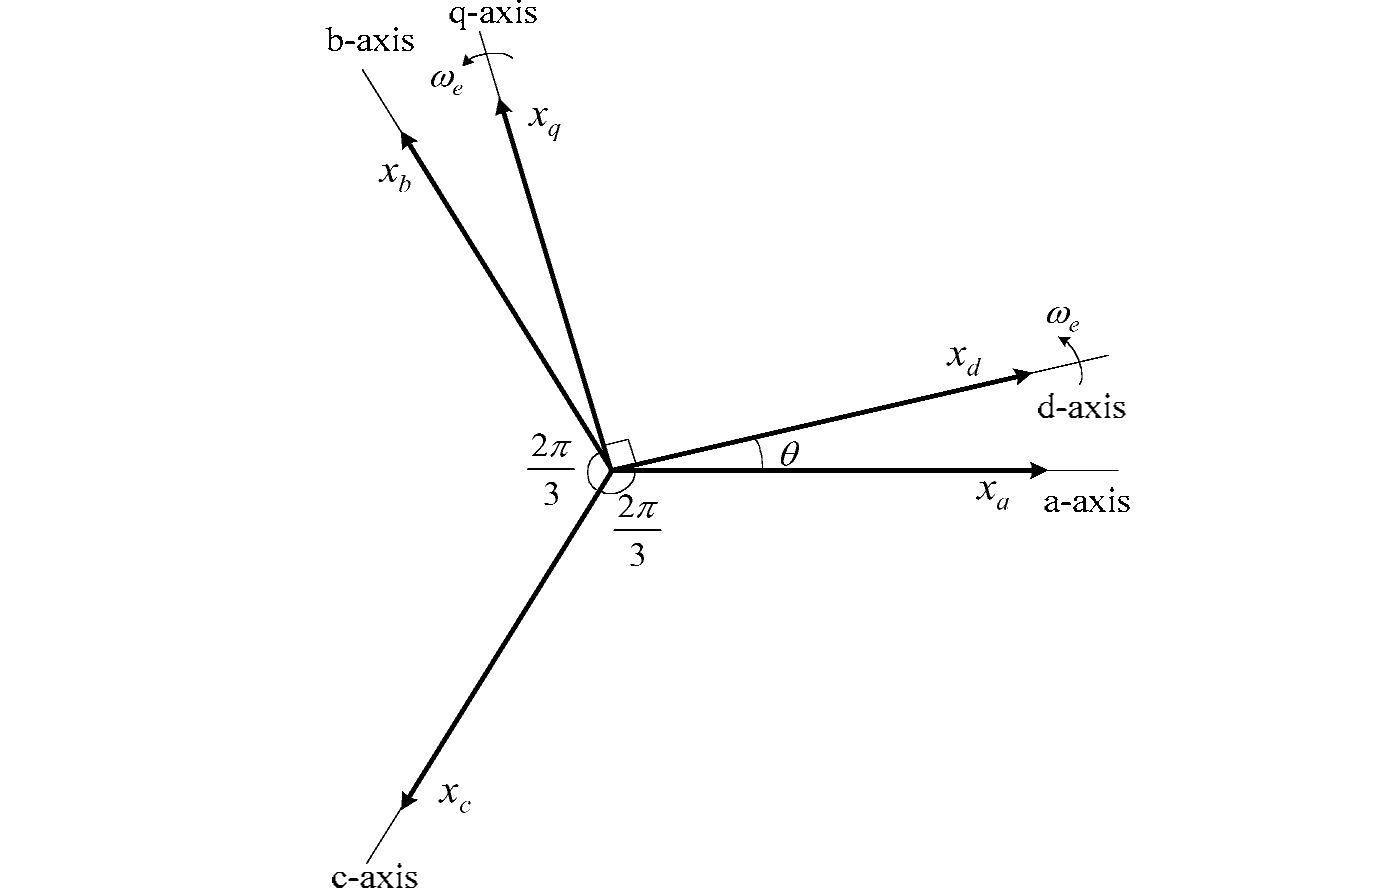
\includegraphics[width=\textwidth]{graficos/img01.jpg} 
    \caption{Figura 14.2-1: Variables en el marco de referencia estacionario de tres fases (abc) y en el marco de referencia síncrono de dos fases (dq).}
    \label{fig:14.2-1}
\end{figure}
\FloatBarrier

Nota que la ecuación de transformación (14.2-1) es válida solo para un sistema balanceado de tres fases, en el cual

\[
    \scalebox{1.5}{$x_a + x_b + x_c = 0 \tag{14.2-4}$}
\]

De manera similar, las variables de dos fases en el marco síncrono pueden transformarse de vuelta al marco estacionario de tres fases mediante

\[
\begin{bmatrix}
x_a \\
x_b \\
x_c 
\end{bmatrix} 
= 
\begin{bmatrix}
\cos \theta & -\sin \theta \\
\cos(\theta - 2\pi/3) & -\sin(\theta - 2\pi/3) \\
\cos(\theta - 4\pi/3) & -\sin(\theta - 4\pi/3)
\end{bmatrix}
\begin{bmatrix}
x_d \\
x_q 
\end{bmatrix} \tag{14.2-5}
\]

lo cual se conoce como transformación dq/abc.

La relación entre un vector de espacio y sus variables de fase se ilustra en la Fig. 14.2-2a, donde un vector de corriente de espacio actual \( \vec{i_s} \) rota a una cierta velocidad \( \omega \) en el marco estacionario (refiérase al Capítulo 6 para la definición del vector de espacio). Sus corrientes de fase \( i_{as}, i_{bs}, \) y \( i_{cs} \) pueden obtenerse descomponiendo \( \vec{i_s} \) en sus respectivos ejes abc. Dado que los tres ejes son estacionarios en el espacio, cada una de las corrientes de fase varía un ciclo completo cuando \( \vec{i_s} \) rota una revolución en el espacio. Si la longitud (magnitud) y la velocidad de rotación de \( \vec{i_s} \) son constantes, las formas de onda de las corrientes de fase a lo largo del tiempo son sinusoidales con un desplazamiento de fase de \( 2\pi/3 \) entre cada una.

La Figura 14.2-2b ilustra otro caso donde el vector de corriente \( \vec{i_s} \) está en el marco de referencia síncrono dq. Suponiendo que \( \vec{i_s} \) rota a la misma velocidad que el marco dq, el ángulo de corriente del estator \( \phi \), que es el ángulo entre \( \vec{i_s} \) y el eje d, es constante. Los componentes de corriente resultantes en el eje dq, \( i_{ds} \) e \( i_{qs} \), son señales de corriente continua. Como se verá en las secciones subsecuentes, esta transformación puede ser utilizada para simplificar la simulación, diseño e implementación digital de sistemas de accionamiento, donde una señal de CA trifásica puede ser representada efectivamente por una señal de CC bifásica.

\begin{figure}[ht]
    \centering
    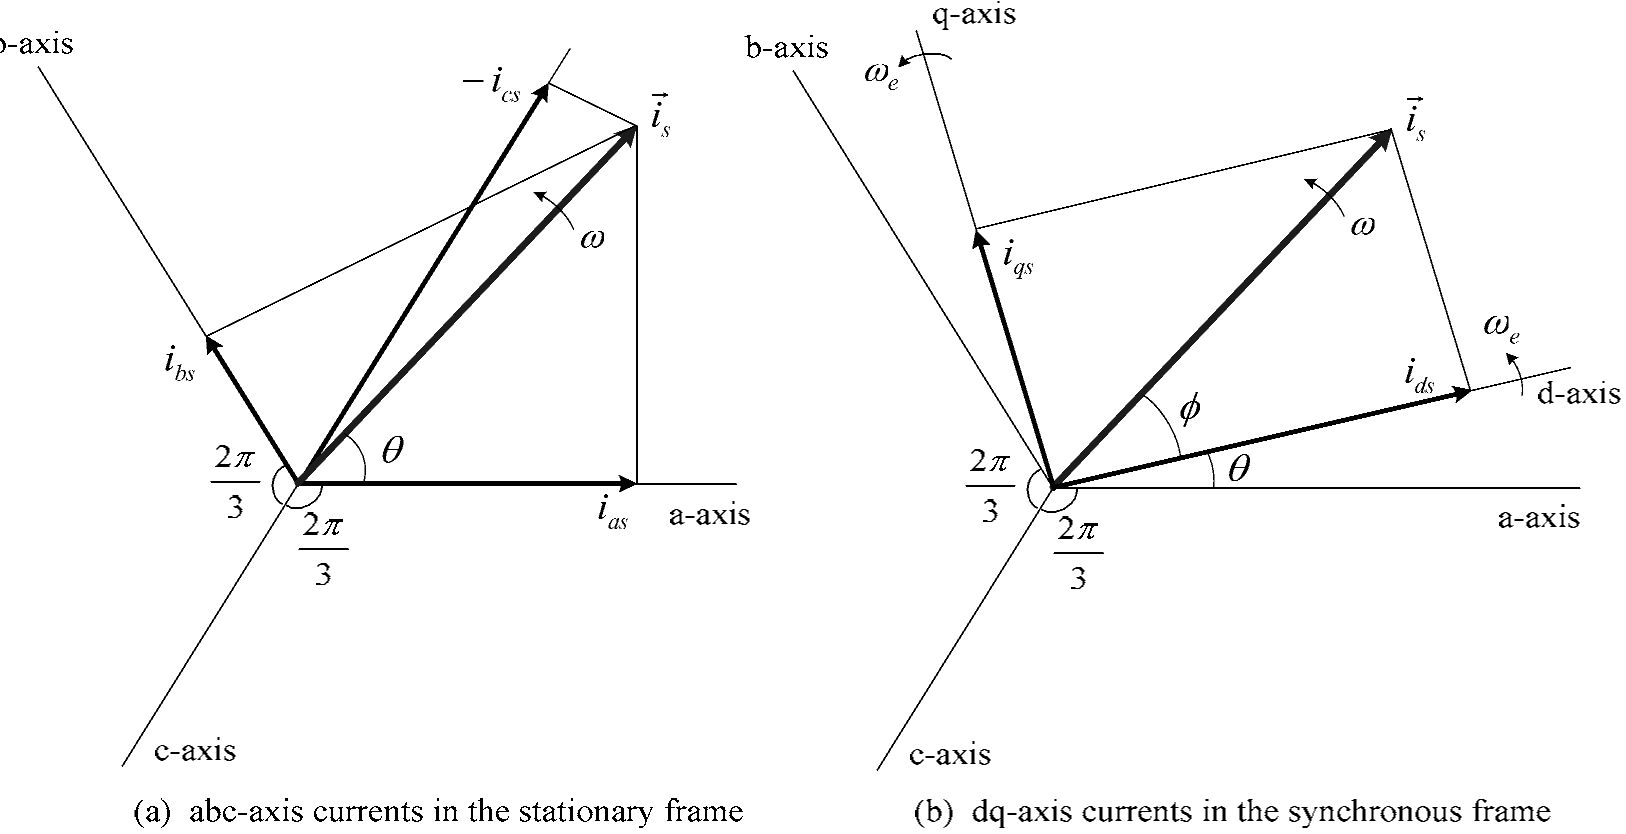
\includegraphics[width=\textwidth]{graficos/img02.jpg} 
    \caption{Figura 14.2-2: Descomposición del vector de corriente \( \vec{i_s} \)}
    \label{fig:14.2-2}
\end{figure}
\FloatBarrier

\subsection{Transformación Estacionaria 3/2}

Con la velocidad de rotación del marco de referencia de dos fases fijada en cero y su eje d coincidiendo con el eje a del marco de tres fases (\(\omega_e = 0\) y \(\theta = 0\)), ambos marcos están estacionarios en el espacio. La transformación de las variables de tres fases a las variables de dos fases puede obtenerse fijando \(\theta\) en (14.2-1) a cero, de la cual

\[
\begin{bmatrix}
x_d \\
x_q 
\end{bmatrix} 
= \frac{2}{3} 
\begin{bmatrix}
1 & -1/2 & -1/2 \\
0 & \sqrt{3}/2 & -\sqrt{3}/2
\end{bmatrix}
\begin{bmatrix}
x_a \\
x_b \\
x_c 
\end{bmatrix} \tag{14.2-6}
\]

La transformación anterior se conoce como transformación 3/2 en este libro. Vale la pena notar que la variable del eje d puede expresarse como

\[
x_d = \frac{2}{3} \left( x_a - \frac{1}{2}x_b - \frac{1}{2}x_c \right) = x_a \tag{14.2-7}
\]

lo cual es igual a la variable del eje a \(x_a\).

De manera similar, la transformación de dos fases a tres fases en el marco estacionario, que se denomina transformación 2/3, puede realizarse mediante

\[
\begin{bmatrix}
x_a \\
x_b \\
x_c 
\end{bmatrix} 
= 
\begin{bmatrix}
1 & 0 \\
-1/2 & \sqrt{3}/2 \\
-1/2 & -\sqrt{3}/2
\end{bmatrix}
\begin{bmatrix}
x_d \\
x_q 
\end{bmatrix} \tag{14.2-8}
\]

\section{Modelos Dinámicos del Motor de Inducción}

Hay dos modelos dinámicos comúnmente usados para el motor de inducción. Uno está basado en la teoría del vector de espacio y el otro se deriva de la teoría del eje dq. El modelo del vector de espacio presenta expresiones matemáticas compactas y diagramas de vectores de espacio concisos, mientras que el modelo del eje dq no necesita usar números o variables complejas. Ambos modelos son igualmente válidos para el análisis del rendimiento transitorio y en estado estacionario del motor de inducción. En lo que sigue, se presentan los dos modelos y se revela su relación.

\subsection{Modelo del Motor de Vector de Espacio}

Se asume en el siguiente análisis que el motor de inducción es simétrico de tres fases y su núcleo magnético es lineal con una pérdida de núcleo despreciable. El modelo para un motor de inducción generalmente se compone de tres conjuntos de ecuaciones [2]. El primer conjunto son las ecuaciones de voltaje, dadas por

\[
\vec{v_s} = R_s \vec{i_s} + p\vec{\lambda_s} + j\omega \vec{\lambda_s}
\]
\[
\vec{v_r} = R_r \vec{i_r} + p\vec{\lambda_r} + j(\omega - \omega_r) \vec{\lambda_r} \tag{14.3-1}
\]

donde \(\vec{v_s}\) y \(\vec{v_r}\) son los vectores de voltaje del estator y del rotor, respectivamente; \(\vec{i_s}\) y \(\vec{i_r}\) son los vectores de corriente del estator y del rotor, respectivamente; \(\vec{\lambda_s}\) y \(\vec{\lambda_r}\) son los vectores de enlace de flujo del estator y del rotor, respectivamente; \(R_s\), \(R_r\) son las resistencias del bobinado del estator y del rotor, respectivamente; \(\omega\) es la velocidad de rotación de un marco de referencia arbitrario; \(\omega_r\) es la velocidad angular del rotor (eléctrica); y \(p\) es el operador derivativo (\(p = d/dt\)).

Los términos \(j\omega \vec{\lambda_s}\) y \(j(\omega - \omega_r) \vec{\lambda_r}\) en el lado derecho de (14.3-1) se denominan voltajes de velocidad, que son inducidos por la rotación del marco de referencia.

El segundo conjunto son las ecuaciones de enlace de flujo

\[
\vec{\lambda_s} = L_s \vec{i_s} + L_m \vec{i_r}
\]
\[
\vec{\lambda_r} = L_r \vec{i_r} + L_m \vec{i_s} \tag{14.3-2}
\]

donde \(L_s = L_{ls} + L_m\) representa la autoinductancia del estator; \(L_r = L_{lr} + L_m\) representa la autoinductancia del rotor; \(L_{ls}\) y \(L_{lr}\) son las inductancias de fuga del estator y del rotor, respectivamente; y \(L_m\) es la inductancia de magnetización. Nótese que todos los parámetros del rotor y las variables, tales como \(R_r\), \(L_{lr}\), \(\vec{i_r}\), y \(\vec{\lambda_r}\), en las ecuaciones anteriores se refieren al lado del estator.

El tercer conjunto es la ecuación de movimiento, dada por

\[
\frac{J}{P} p \omega_r = T_e - T_L
\]
\[
T_e = \frac{3P}{2} \text{Re} (\vec{J} \vec{\lambda_s} \vec{i_s}^*) = -\frac{3P}{2} \text{Re} (\vec{J} \vec{\lambda_r} \vec{i_r}^*) \tag{14.3-3}
\]

donde \(J\) es el momento total de inercia del rotor y la carga, \(P\) es el número de pares de polos, \(T_L\) es el par de carga, y \(T_e\) es el par electromagnético.

Las ecuaciones anteriores constituyen el modelo de vector de espacio del motor de inducción cuya representación esquemática se da en la Fig. 14.3-1. El modelo del motor está en el marco de referencia arbitrario que rota en el espacio a la velocidad arbitraria \(\omega\).

\begin{figure}[ht]
    \centering
    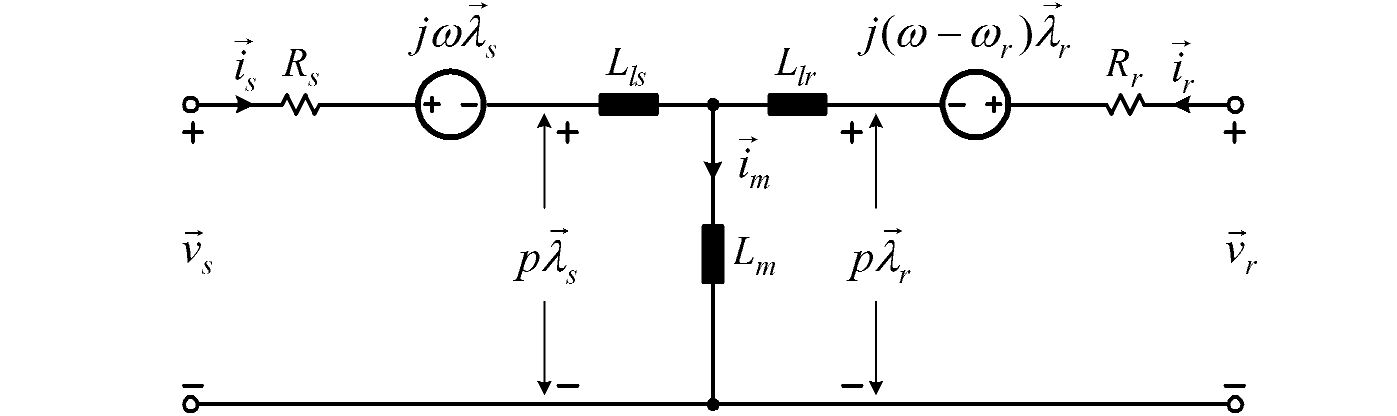
\includegraphics{graficos/img03.jpg} 
    \caption{Figura 14.3-1: Modelo de vector de espacio de un motor de inducción en el marco de referencia arbitrario.}
    \label{fig:14.3-1}
\end{figure}
\FloatBarrier

En la simulación e implementación digital de sistemas de control avanzados, los modelos de motor en los marcos de referencia síncrono y estacionario se emplean a menudo. El modelo de motor en el marco síncrono puede obtenerse fácilmente fijando la velocidad arbitraria \(\omega\) en (14.3-1) a la velocidad síncrona \(\omega_e\). La Figura 14.3-2a muestra el circuito equivalente de un motor de jaula de ardilla en el marco síncrono, donde el bobinado del rotor está en cortocircuito (\(\vec{v_r} = 0\)) y \(\omega_{sl}\) es la frecuencia de deslizamiento angular, dada por

\[
\omega_{sl} = \omega_e - \omega_r \tag{14.3-4}
\]

Para obtener el modelo en el marco estacionario (del estator), podemos fijar la velocidad arbitraria \(\omega\) del marco de referencia rotatorio a cero. El circuito equivalente resultante se muestra en la Fig. 14.3-2b.

\begin{figure}[ht]
    \centering
    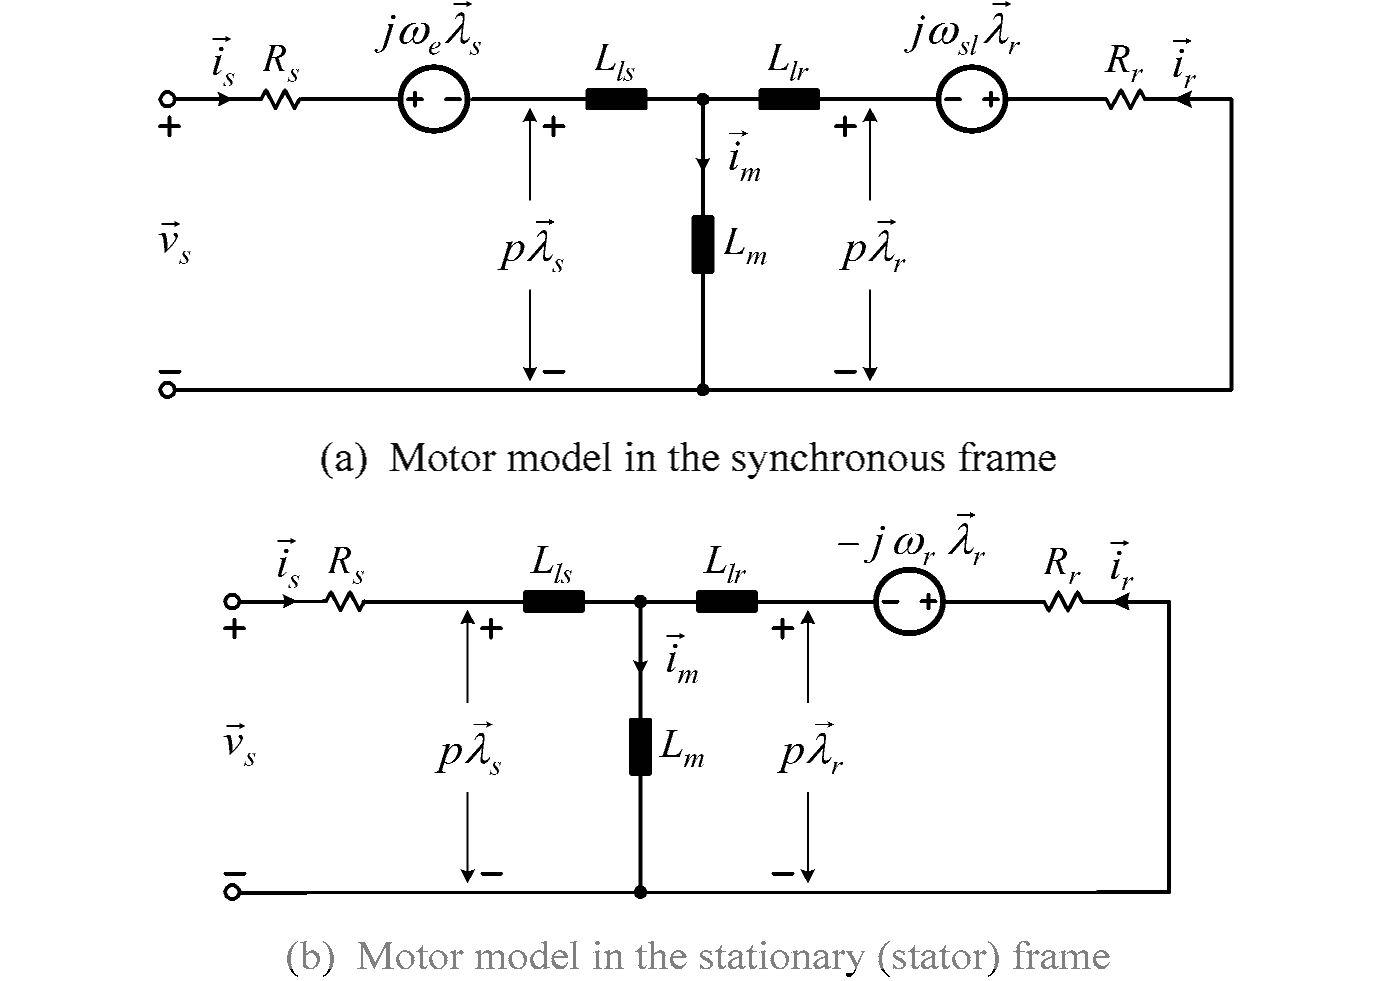
\includegraphics{graficos/img04.jpg} 
    \caption{Figura 14.3-2: Modelos de vector de espacio para un motor de inducción de jaula de ardilla.}
    \label{fig:14.3-2}
\end{figure}
\FloatBarrier

\subsection{Modelo del Motor en el Eje dq}

El modelo del motor de inducción en el eje dq puede derivarse usando la teoría de circuitos de tres fases y luego transformarse al marco de dos fases (eje dq) [1]. Alternativamente, puede


también puede obtenerse descomponiendo los vectores de espacio en el modelo de motor de vector de espacio en los componentes de los ejes d y q [2], es decir,

\[
\vec{v_s} = v_{ds} + jv_{qs}, \quad \vec{i_s} = i_{ds} + ji_{qs}, \quad \vec{\lambda_s} = \lambda_{ds} + j\lambda_{qs}
\]
\[
\vec{v_r} = v_{dr} + jv_{qr}, \quad \vec{i_r} = i_{dr} + ji_{qr}, \quad \vec{\lambda_r} = \lambda_{dr} + j\lambda_{qr} \tag{14.3-5}
\]

Sustituyendo (14.3-5) en (14.3-1), se pueden obtener las ecuaciones de voltaje en el eje dq para el motor de inducción:

\[
v_{ds} = R_s i_{ds} + p\lambda_{ds} - \omega \lambda_{qs}
\]
\[
v_{qs} = R_s i_{qs} + p\lambda_{qs} + \omega \lambda_{ds}
\]
\[
v_{dr} = R_r i_{dr} + p\lambda_{dr} - (\omega - \omega_r) \lambda_{dr}
\]
\[
v_{qr} = R_r i_{qr} + p\lambda_{qr} + (\omega - \omega_r) \lambda_{qr} \tag{14.3-6}
\]

donde los enlaces de flujo del estator y del rotor pueden calcularse mediante

\[
\lambda_{ds} = L_s i_{ds} + L_m (i_{ds} + i_{dr})
\]
\[
\lambda_{qs} = L_s i_{qs} + L_m (i_{qs} + i_{qr})
\]
\[
\lambda_{dr} = L_r i_{dr} + L_m (i_{ds} + i_{dr})
\]
\[
\lambda_{qr} = L_r i_{qr} + L_m (i_{qs} + i_{qr}) \tag{14.3-7}
\]

El par electromagnético puede expresarse de varias maneras. Algunas de las expresiones comúnmente utilizadas son

\[
T_e = \left\{
\begin{array}{l}
\frac{3P}{2} (i_{qs}\lambda_{ds} - i_{ds}\lambda_{qs}) \\
\frac{3P L_m}{2} (i_{qs} i_{dr} - i_{ds} i_{qr}) \\
\frac{3P L_m}{2L_r} (i_{qs} \lambda_{dr} - i_{ds} \lambda_{qr})
\end{array}
\right\} \tag{14.3-8}
\]

Las ecuaciones (14.3-6) a (14.3-8) junto con la ecuación de movimiento de (14.3-3) representan el modelo de eje dq del motor de inducción, cuyo circuito equivalente se muestra en la Fig. 14.3-3.

\subsection{Características Transitorias del Motor de Inducción}

Es instructivo estudiar las características transitorias del motor de inducción durante la aceleración libre utilizando los modelos dinámicos del motor. El motor bajo investigación es un motor de jaula de ardilla de baja potencia con los siguientes parámetros: \(V_{LL} = 208 \text{V}, 60\text{ Hz}, Z_{base} = 15.4 \, \Omega, R_s = 0.068 \, pu, R_r = 0.045 \, pu, L_{ls} = L_{lr} = 0.058 \, pu, L_m = 1.95 \, pu, P = 1, J = 0.02 \, kg \cdot m^2\). La Figura 14.3-4 muestra el diagrama de bloques para la simulación por computadora con el modelo del motor en el marco estacionario (\(\omega = 0\)). Los voltajes de suministro trifásicos \(v_{as}\), \(v_{bs}\), y \(v_{cs}\) se transforman en los voltajes del estator en el eje dq \(v_{ds}\) y \(v_{qs}\) mediante la transformación 3/2. Las corrientes simuladas del estator en el eje dq \(i_{ds}\) e \(i_{qs}\) se convierten luego en las corrientes trifásicas \(i_{as}\), \(i_{bs}\), y \(i_{cs}\) mediante la transformación 2/3.

\begin{figure}[ht]
    \centering
    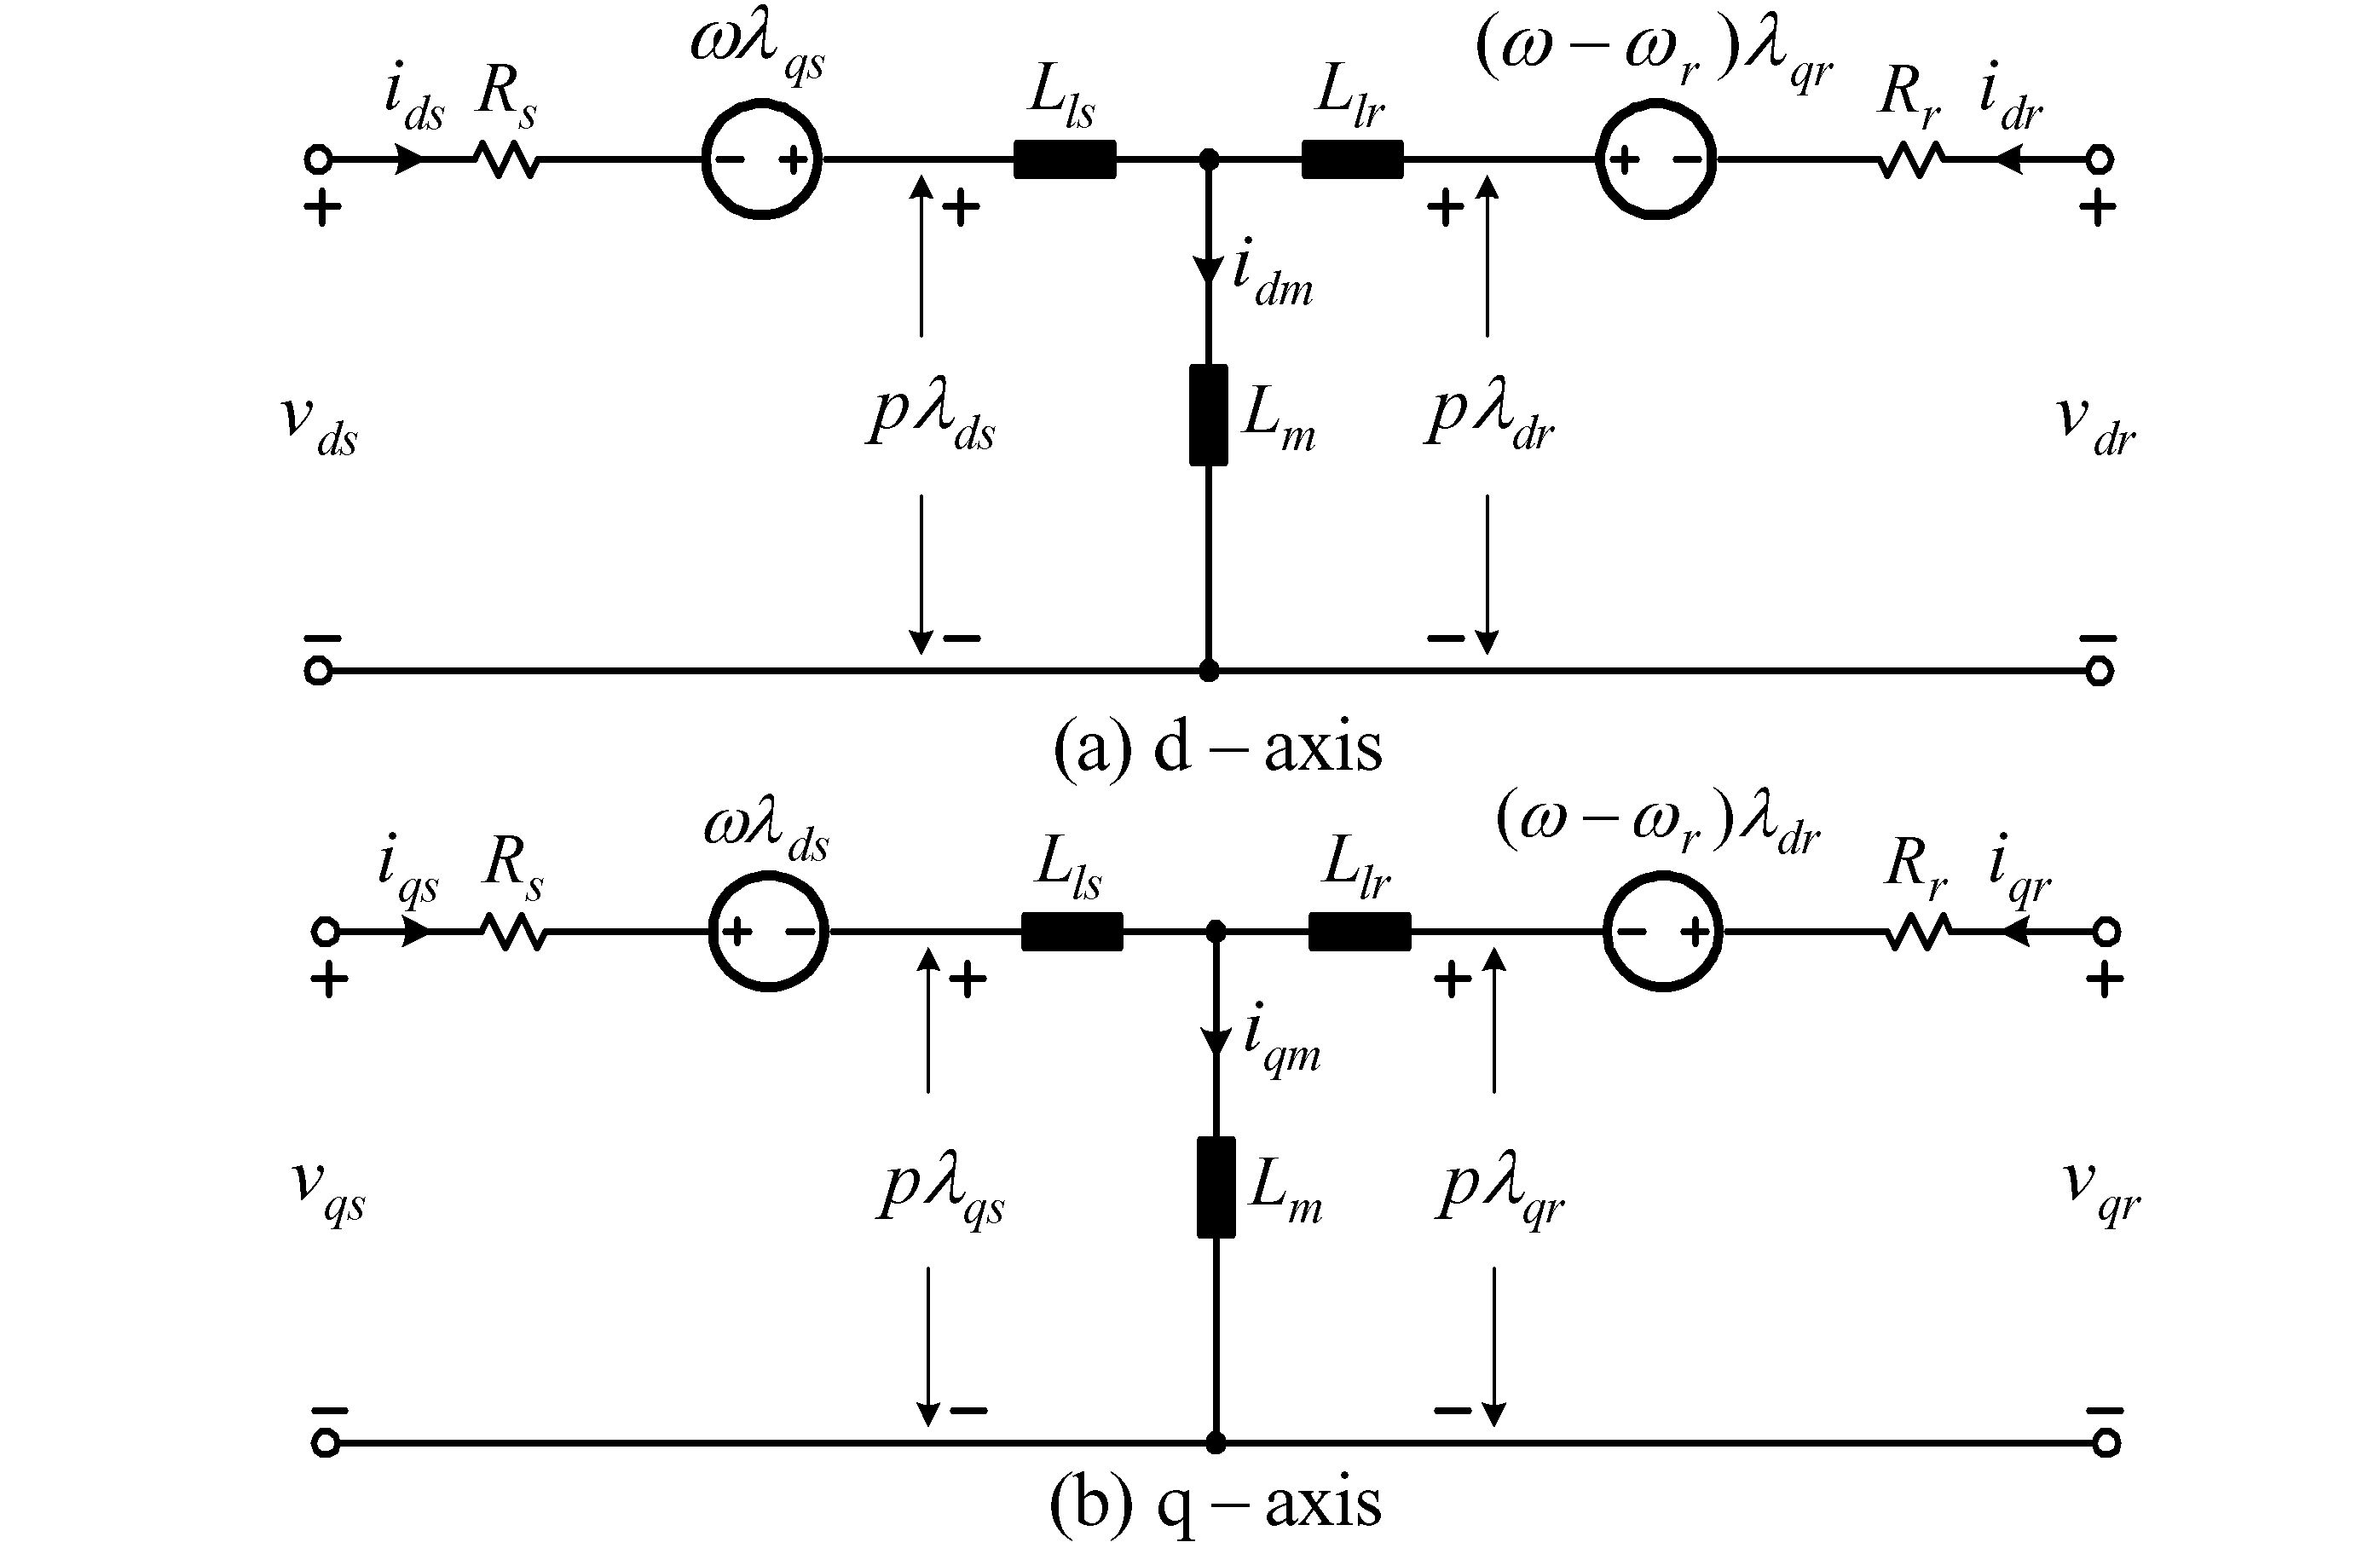
\includegraphics{graficos/img05.jpg} 
    \caption{Figura 14.3-4: Diagrama de bloques para la simulación de la aceleración libre del motor usando el modelo del motor en el marco estacionario.}
    \label{fig:14.3-4}
\end{figure}
\FloatBarrier  

La Figura 14.3-5a muestra las formas de onda transitorias simuladas de la corriente del estator \(i_{as}\) y la velocidad del rotor \(n_r\) durante la aceleración libre del motor (el motor arranca bajo los voltajes nominales de voltaje y frecuencia sin carga mecánica). La velocidad del rotor \(n_r\), en rpm, se relaciona con la velocidad angular eléctrica del rotor \(\omega_r\) por

\[
    \scalebox{1.5}{$n_r = \frac{30}{\pi P} \omega_r \tag{14.3-9}$}
\]

La corriente de arranque pico es aproximadamente 8.4 pu, lo que representa la corriente de arranque rms de 5.9 pu. El tiempo de arranque es de alrededor de 0.5 s debido al bajo momento de inercia y la alta corriente de arranque. Las formas de onda medidas durante la aceleración libre se muestran en la Figura 14.3-5b, las cuales coinciden muy bien con los resultados simulados.

\begin{figure}[ht]
    \centering
    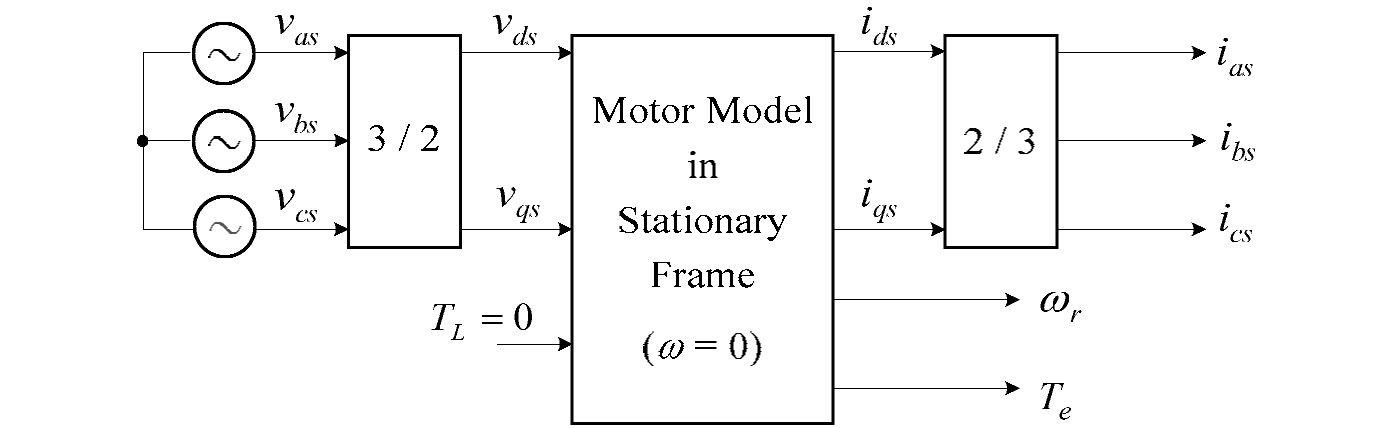
\includegraphics{graficos/img06.jpg} 
    \caption{Figura 14.3-5: Formas de onda de un motor de inducción durante la aceleración libre. (a) Formas de onda simuladas, (b) Formas de onda medidas.}
    \label{fig:14.3-5}
\end{figure}
\FloatBarrier  

La Figura 14.3-6 muestra formas de onda transitorias simuladas y medidas del motor durante una falla de tres fases. El motor opera cerca de su velocidad síncrona cuando sus terminales de tres fases están cortocircuitadas. La corriente pico máxima del estator es cercana a la de la aceleración libre. Las formas de onda medidas se correlacionan estrechamente con las simuladas.

\begin{figure}[ht]
    \centering
    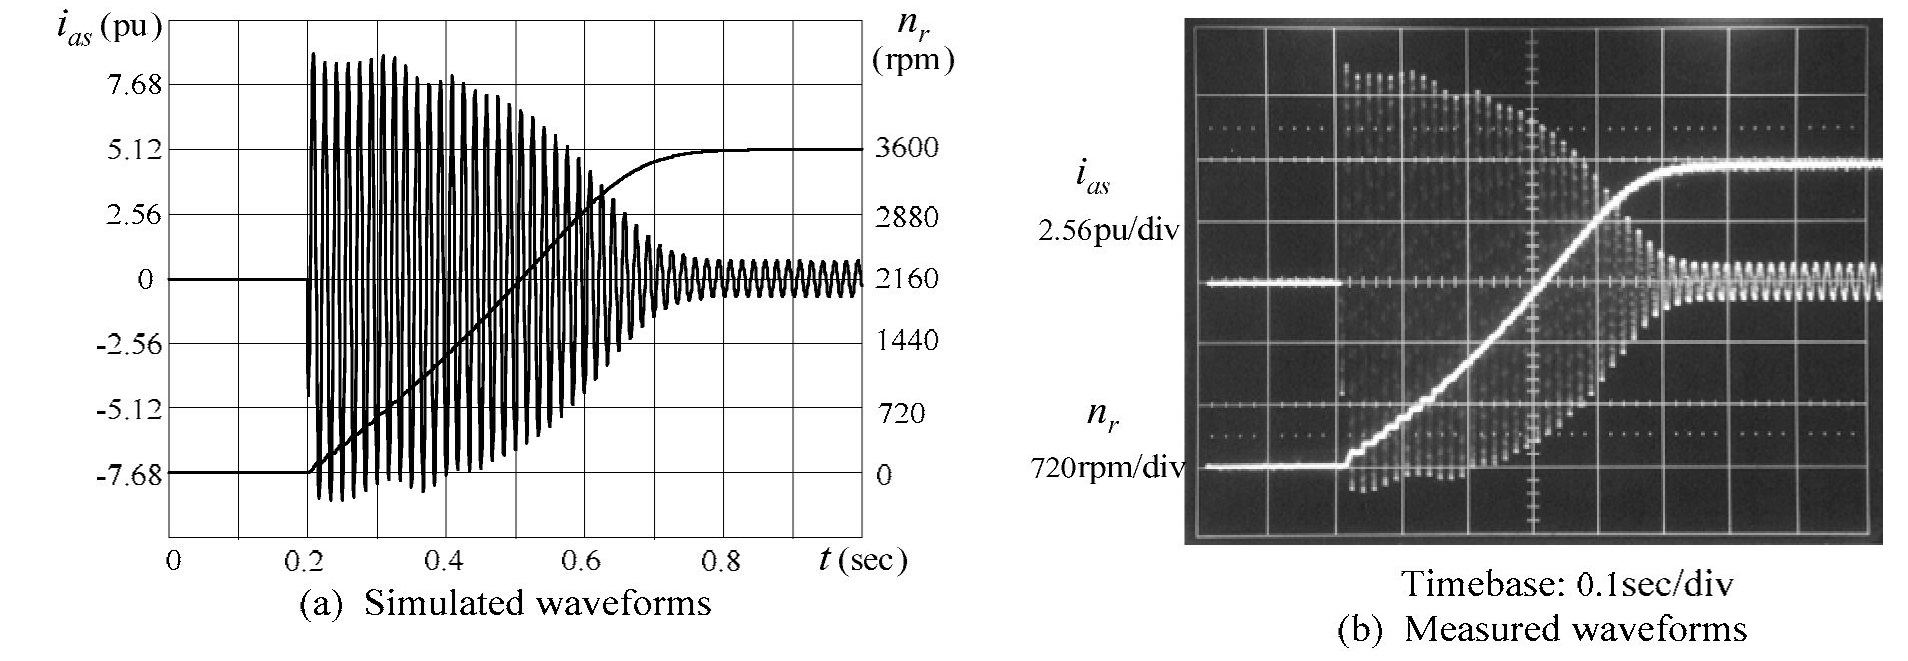
\includegraphics{graficos/img07.jpg} 
    \caption{Figura 14.3-6: Formas de onda de corriente del estator de un motor de inducción durante una falla de tres fases.}
    \label{fig:14.3-6}
\end{figure}
\FloatBarrier

La Figura 14.3-7 ilustra el diagrama de bloques de simulación con el modelo de motor en el marco síncrono. Usando los bloques de transformación abc/dq y dq/abc, los voltajes de suministro trifásicos \(v_{as}\), \(v_{bs}\) y \(v_{cs}\) en el marco estacionario pueden transformarse a los voltajes del estator en el eje dq \(v_{ds}\) y \(v_{qs}\) en el marco síncrono, mientras que las corrientes simuladas del estator en el eje dq \(i_{ds}\) e \(i_{qs}\) en el marco síncrono pueden convertirse en corrientes trifásicas \(i_{as}\), \(i_{bs}\) e \(i_{cs}\) en el marco estacionario. El ángulo \(\theta\) en los bloques de transformación puede obtenerse mediante la transformación 3/2 y los bloques de arctangente \(\tan^{-1}\) como se muestra en la figura o usando la Ecuación (14.2-3) directamente.

\begin{figure}[ht]
    \centering
    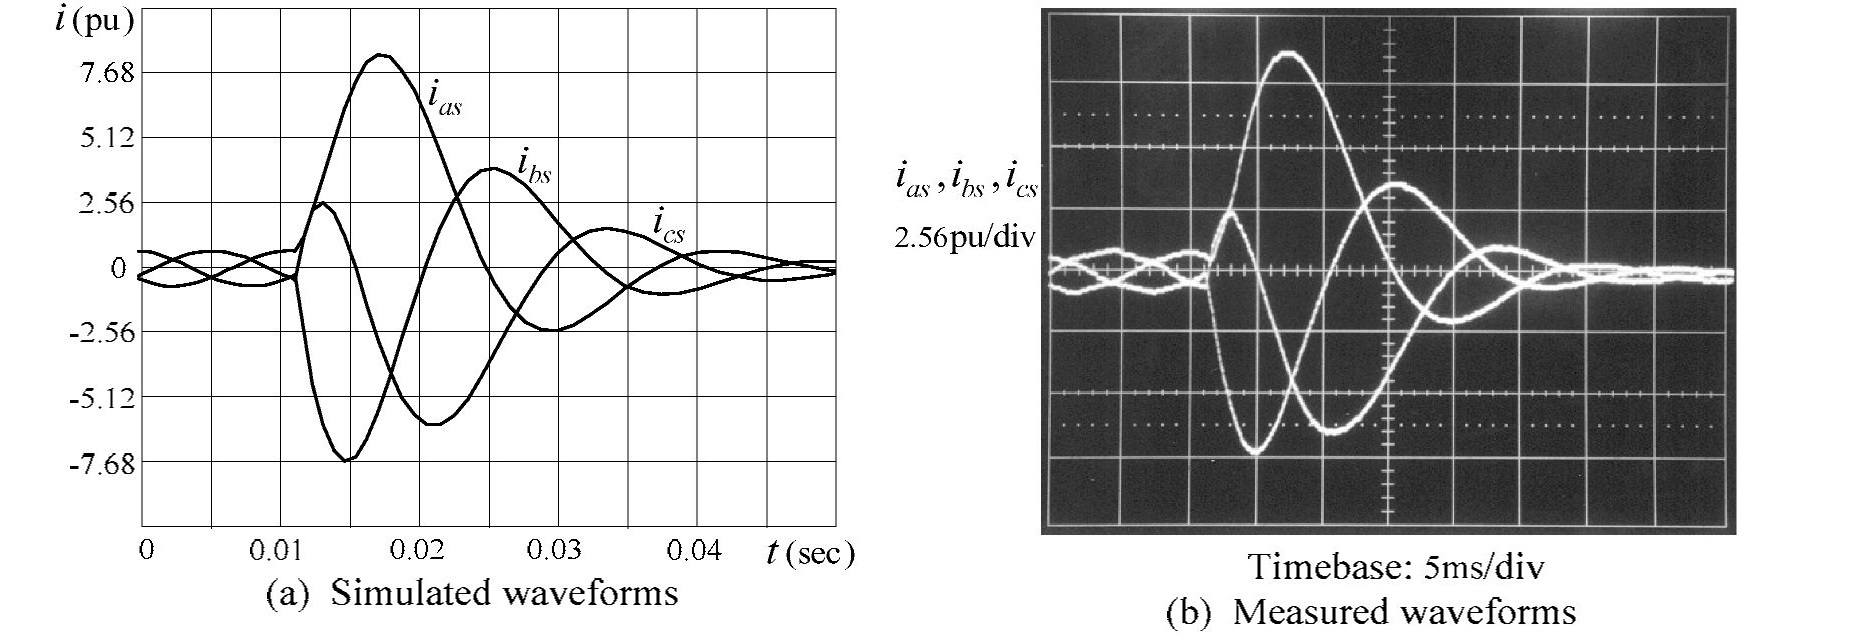
\includegraphics{graficos/img08.jpg} 
    \caption{Figura 14.3-7: Diagrama de bloques para la simulación de la aceleración libre del motor usando el modelo de motor en el marco síncrono.}
    \label{fig:14.3-7}
\end{figure}
\FloatBarrier

La Figura 14.3-8a muestra las formas de onda simuladas de las corrientes \(i_{as}\), \(i_{ds}\) e \(i_{qs}\) durante la aceleración libre del motor. La forma de onda para \(i_{as}\) en el marco estacionario es exactamente la misma que en la Fig. 14.3-5. Las corrientes en el eje dq \(i_{ds}\) e \(i_{qs}\) están en el marco síncrono y, por lo tanto, son señales de corriente continua en estado estacionario. La amplitud de la corriente del estator \( \vec{i_s} \) puede obtenerse mediante \( \vec{i_s} = \sqrt{i_{ds}^2 + i_{qs}^2} \). Los voltajes del eje dq \(v_{ds}\) y \(v_{qs}\) en el marco síncrono son de corriente continua constante y, por lo tanto, no se muestran en la figura.

\begin{figure}[ht]
    \centering
    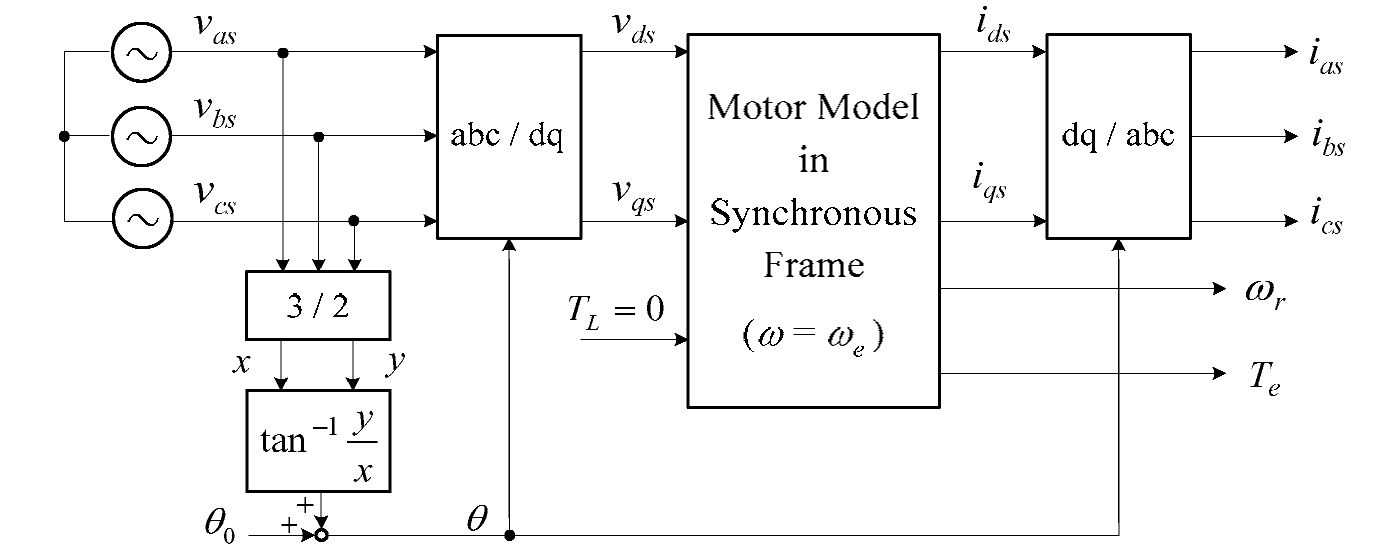
\includegraphics{graficos/img09.jpg} 
    \caption{Figura 14.3-8: Formas de onda simuladas para la aceleración libre del motor usando el modelo de motor en el marco síncrono. (a) Corrientes, (b) Par.}
    \label{fig:14.3-8}
\end{figure}
\FloatBarrier

La corriente del estator ángulo \( \phi \), que es el ángulo entre \( \vec{i_s} \) y el eje d como se muestra en la Fig. 14.2-2b, afectará las formas de onda de \( i_{ds} \) e \( i_{qs} \). Las formas de onda en la Fig. 14.3-8a se obtienen con \( \phi = 0 \) ajustando el ángulo inicial \(\theta_0\) de modo que el eje d del marco síncrono esté alineado con \( \vec{i_s} \). Esto lleva a \( i_{qs} = 0 \) e \( i_{ds} = i_s \), cuando el motor está en operación en estado estacionario. Si el eje q del marco síncrono está alineado con \( \vec{i_s} \) (\( \phi = 90^\circ \)), las corrientes en estado estacionario en el eje dq son \( i_{qs} = i_s \) e \( i_{ds} = 0 \). Sin embargo, la forma de onda de \( i_s \) no se ve afectada por \( \phi \).

La respuesta del par durante la aceleración libre del motor se muestra en la Fig. 14.3-8b. Aunque se obtiene con el modelo del motor en el marco síncrono, la respuesta permanece igual para el modelo del motor en cualquier otro marco de referencia.

\section{Principio del Control Orientado al Campo (FOC)}

\subsection{Orientación del Campo}

Es bien conocido que el accionamiento del motor de corriente continua tiene un excelente rendimiento dinámico. Esto se debe principalmente al control desacoplado (separado) del campo magnético del estator y el par electromagnético del motor. El par se desarrolla por la interacción de dos campos magnéticos perpendiculares. Un campo es generado por la corriente de campo \( i_f \) en el devanado del estator, y el otro es producido por la corriente de armadura (rotor) \( i_a \). El par desarrollado puede expresarse como

\[
\scalebox{1.5}{$T_e = K_a \lambda_f i_a$} \tag{14.4-1}
\]

donde \( K_a \) es una constante de armadura y \( \lambda_f \) es el flujo producido por \( i_f \). En los accionamientos de corriente continua de alto rendimiento, \( \lambda_f \) normalmente se mantiene constante manteniendo \( i_f \) constante, y por lo tanto, el par \( T_e \) es proporcional a \( i_a \) y puede ser controlado directamente por \( i_a \).

El control orientado al campo, también conocido como control vectorial, para el motor de inducción emula el control del motor de corriente continua. Usando una orientación de campo adecuada, la corriente del estator puede descomponerse en un componente de producción de flujo y un componente de producción de par. Estos dos componentes luego se controlan por separado.

La orientación del campo puede clasificarse generalmente en orientación del flujo del estator, flujo del entrehierro y orientación del flujo del rotor [3, 4]. Dado que la orientación del flujo del rotor se usa extensamente en los accionamientos de corriente alterna, este esquema se analizará en detalle. Su principio de operación puede aplicarse fácilmente a los otros dos esquemas de orientación del campo.

La orientación del flujo del rotor se logra alineando el eje d del marco de referencia síncrono con el vector de flujo del rotor \( \vec{\lambda_r} \), como se muestra en la Fig. 14.4-1. Los componentes resultantes del flujo del rotor en los ejes d y q son

\[
\scalebox{1.5}{$\lambda_{qr} = 0 \quad \text{y} \quad \lambda_{dr} = \lambda_r$} \tag{14.4-2}
\]

donde \( \lambda_r \) es la magnitud de \( \vec{\lambda_r} \). Sustituyendo (14.4-2) en la última ecuación de (14.3-8) se obtiene

\[
\scalebox{1.5}{$T_e = K_r \lambda_r i_{qs} = K_r \lambda_r i_{qs}$} \tag{14.4-3}
\]


\begin{figure}[ht]
    \centering
    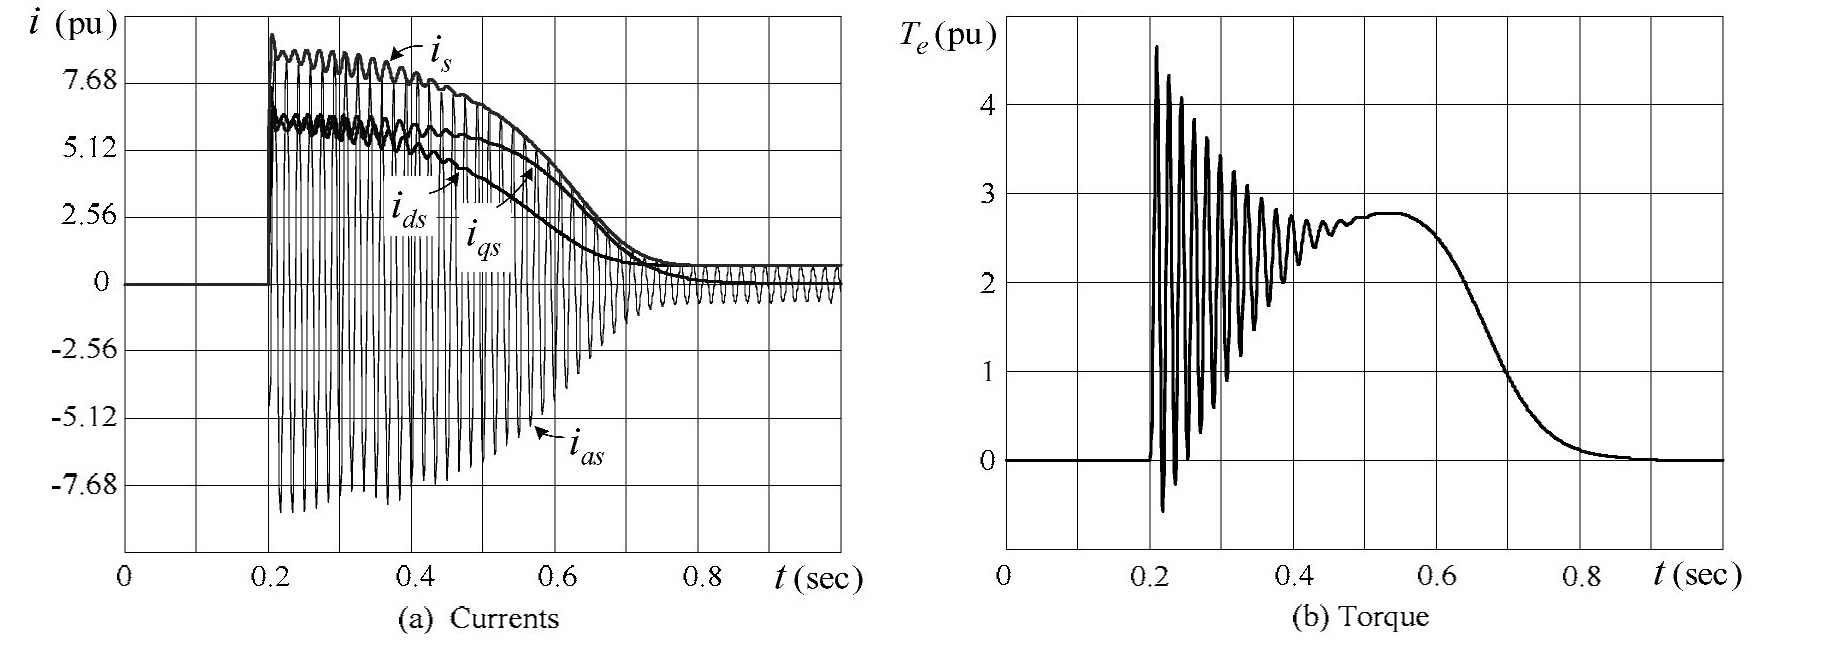
\includegraphics{graficos/img10.jpg} 
    \caption{Figura 14.4-1: Orientación del campo de flujo del rotor (el eje d está alineado con \( \vec{\lambda_r} \)).}
    \label{fig:14.4-1}
\end{figure}
\FloatBarrier

donde \( K_r = \frac{3P L_m}{2 L_r} \). La Ecuación (14.4-3) indica que con la orientación del campo del rotor, la expresión del par para el motor de inducción es similar a la de un motor de corriente continua. Si \( \lambda_r \) se puede mantener constante durante la operación del motor, el par desarrollado se puede controlar directamente por la corriente del estator en el eje q \( i_{qs} \).

El vector de corriente del estator \( \vec{i_s} \) en la Fig. 14.4-1 se puede resolver en dos componentes a lo largo de los ejes dq. La corriente en el eje d \( i_{ds} \) se refiere a la corriente productora de flujo, mientras que la corriente en el eje q \( i_{qs} \), que es perpendicular a \( i_{ds} \), es la corriente productora de par. En el control orientado al campo, \( i_{ds} \) normalmente se mantiene en su valor nominal, mientras que \( i_{qs} \) se controla independientemente. Con el control desacoplado para \( i_{ds} \) e \( i_{qs} \), se puede realizar un accionamiento de alto rendimiento.

Uno de los problemas clave asociados con el control orientado al flujo del rotor es determinar con precisión el ángulo de flujo del rotor \( \theta_f \) para la orientación del campo. Se pueden usar varios esquemas para encontrar \( \theta_f \). Por ejemplo, se puede calcular a partir de las tensiones y corrientes medidas del estator, o se puede encontrar a partir de

\[
\scalebox{1.25}{$\theta_f = \theta_r + \theta_{sl}$} \tag{14.4-4}
\]

donde \( \theta_r \) y \( \theta_{sl} \) son el ángulo de posición del rotor medido y el ángulo de deslizamiento calculado, respectivamente.

\subsection{Diagrama de Bloques General del FOC}

Dependiendo de cómo se obtenga el ángulo de flujo del rotor \( \theta_f \), los esquemas de control se pueden clasificar en control orientado al campo directo e indirecto. Si \( \theta_f \) se obtiene utilizando dispositivos de detección de flujo incrustados dentro del motor o utilizando tensiones y corrientes terminales medidas del motor, el método se conoce como control orientado al campo directo. Si el ángulo de flujo del rotor \( \theta_f \) se obtiene a partir del ángulo de posición del rotor detectado \( \theta_r \) y el ángulo de deslizamiento calculado \( \theta_{sl} \) como se muestra en (14.4-4), este esquema se conoce como control orientado al campo indirecto.

Un diagrama de bloques general de un accionamiento de motor de inducción con control orientado al flujo del rotor se muestra en la Fig. 14.4-2. Dado que la esencia del FOC es el control desacoplado del flujo del rotor \( \lambda_r \) y el par electromagnético \( T_e \), estas dos variables se controlan por separado. La referencia de par \( T_e^* \) es generada por el Controlador de Velocidad basado en la velocidad de referencia \( \omega_r^* \) y la velocidad del rotor detectada o estimada \( \omega_r \). La referencia de flujo del rotor \( \lambda_r^* \) es una función de \( \omega_r^* \). Cuando el motor opera a su velocidad nominal o por debajo de ella, \( \lambda_r^* \) normalmente se mantiene en su valor nominal. Con la velocidad nominal superada, \( \lambda_r^* \) debe debilitarse en consecuencia para que la tensión del estator y la potencia de salida del motor no excedan sus valores nominales.

Las dos referencias \( \lambda_r^* \) y \( T_e^* \) se envían al Controlador de Flujo/Par, donde se comparan con el flujo del rotor calculado \( \lambda_r \) y el par \( T_e \) para un control en lazo cerrado. El Controlador de Flujo/Par genera señales de referencia para el bloque PWM, que produce señales de compuerta para el inversor para ajustar su tensión y frecuencia de salida.

\begin{figure}[ht]
    \centering
    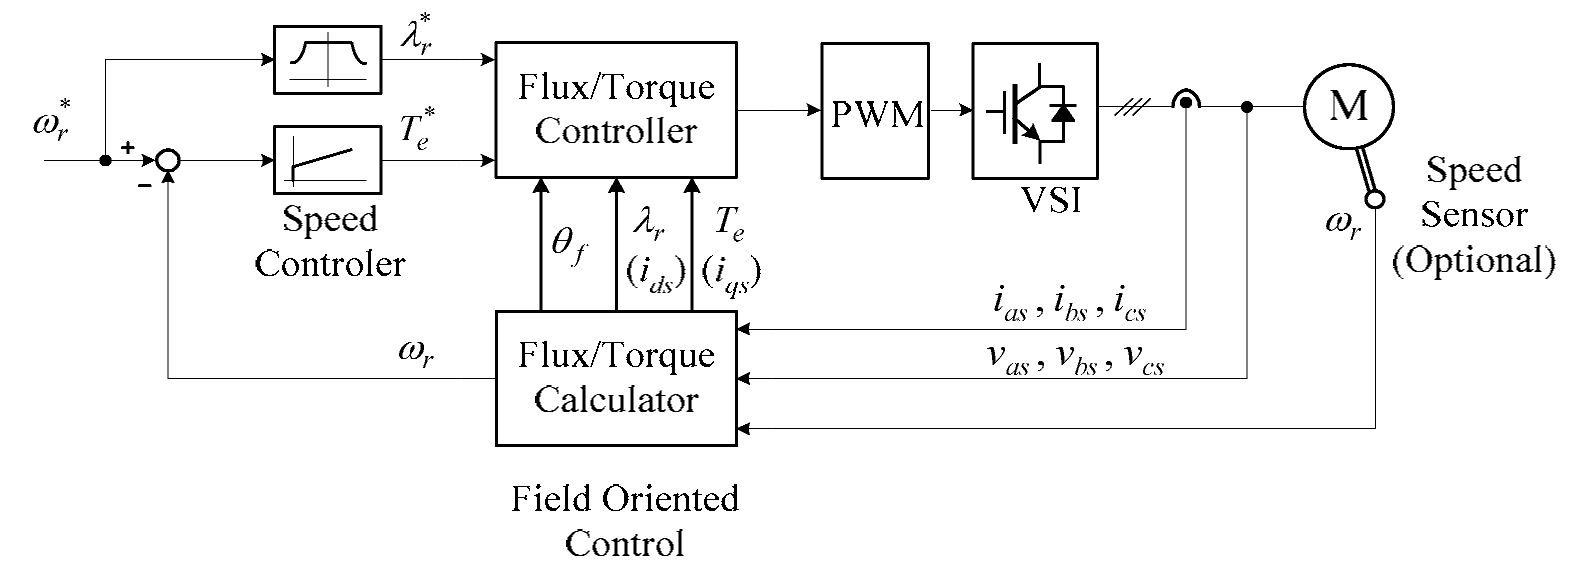
\includegraphics{graficos/img12.jpg} 
    \caption{Figura 14.4-2: Diagrama de bloques general del FOC de flujo del rotor.}
    \label{fig:14.4-2}
\end{figure}
\FloatBarrier

Basado en las variables de tensión y corriente del estator medidas y el modelo del motor, el Calculador de Flujo/Par calcula (1) el ángulo de flujo del rotor \( \theta_f \) para la orientación del campo, (2) la magnitud del flujo del rotor \( \lambda_r \) o la corriente productora de flujo \( i_{ds} \), (3) el par electromagnético \( T_e \) o la corriente productora de par \( i_{qs} \), y (4) la velocidad del rotor \( \omega_r \). Dependiendo de los requisitos del sistema de accionamiento y el tipo de esquema FOC empleado, la velocidad del rotor \( \omega_r \) también puede ser detectada directamente por un sensor de velocidad digital. Cabe destacar que el Calculador de Flujo/Par, también conocido como Observador de Flujo/Par o Estimador en la literatura, es el bloque funcional más importante en el esquema FOC.

\section{Control Orientado al Campo Directo}

\subsection{Diagrama de Bloques del Sistema}

La Figura 14.5-1 muestra un diagrama de bloques típico del control orientado al campo directo para un motor de inducción, donde no se muestra el control de velocidad del rotor por simplicidad. Hay tres bucles de control de retroalimentación, uno para el enlace de flujo del rotor \( \lambda_r \), otro para la corriente del estator en el eje d \( i_{ds} \) (productora de flujo), y otro para la corriente del estator en el eje q \( i_{qs} \) (productora de par).

Para el control del flujo del rotor, la \( \lambda_r \) calculada se compara con su referencia \( \lambda_r^* \) para generar la referencia de corriente del estator en el eje d \( i_{ds}^* \) a través del controlador de flujo (FC). La referencia de corriente del estator en el eje q \( i_{qs}^* \) se genera según la referencia de par \( T_e^* \). Las corrientes de retroalimentación del estator en el eje dq \( i_{ds} \) e \( i_{qs} \) se comparan con sus referencias, y los errores se envían a los controladores de corriente para generar las referencias de tensión del estator \( v_{ds}^* \) y \( v_{qs}^* \). Las tensiones del estator en el eje dq en el marco síncrono se transforman luego en las tensiones del estator trifásicas \( v_{as}^* \), \( v_{bs}^* \), y \( v_{cs}^* \) en el marco estacionario para el bloque PWM. Se pueden usar varios esquemas de PWM. Si se emplea un esquema de modulación basado en portadoras, \( v_{as}^* \), \( v_{bs}^* \), y \( v_{cs}^* \) son las señales moduladoras que se comparan con una onda portadora triangular para generar las señales de compuerta PWM para los dispositivos de conmutación en el inversor.

Como se muestra en la Fig. 14.5-1, el ángulo de flujo del rotor \( \theta_f \) se usa en los bloques de transformación abc/dq y dq/abc para la orientación del campo. Las variables a la izquierda de los bloques de transformación son todas señales de corriente continua en el marco síncrono, mientras que las del lado derecho de los bloques de transformación son todas variables de corriente alterna en el marco estacionario.

\begin{figure}[ht]
    \centering
    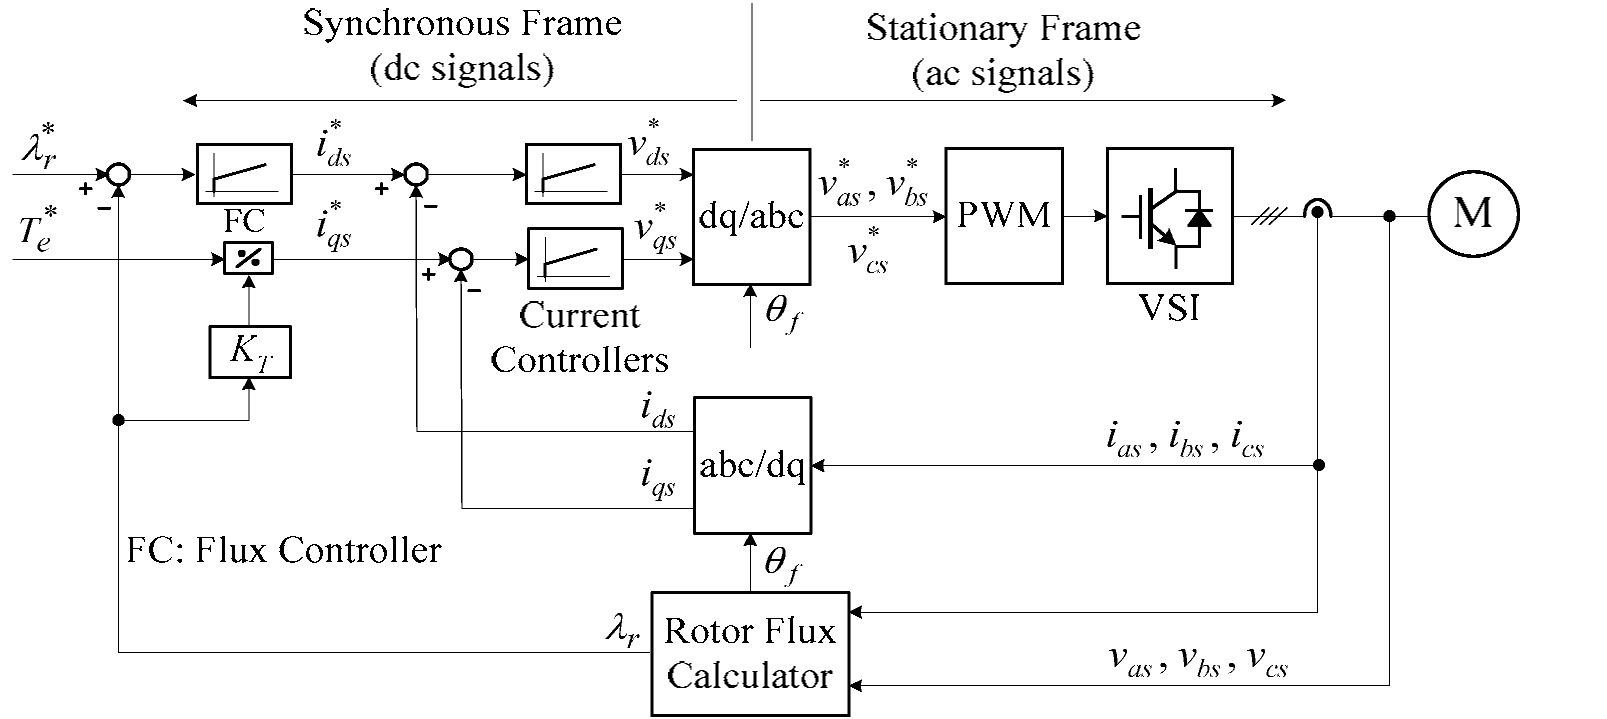
\includegraphics{graficos/img13.jpg} 
    \caption{Figura 14.5-1: Control orientado al campo directo con orientación del flujo del rotor.}
    \label{fig:14.5-1}
\end{figure}
\FloatBarrier

\subsection{Calculador de Flujo del Rotor}

Basado en el modelo del motor en el marco estacionario en la Fig. 14.3-2b, el vector de flujo del estator se puede expresar como

\[
\scalebox{1.25}{$\vec{\lambda_s} = \int (\vec{v_s} - R_s \vec{i_s}) \, dt$} \tag{14.5-1}
\]

El vector de flujo del rotor se puede encontrar a partir de las ecuaciones de enlace de flujo (14.3-2):

\[
\scalebox{1.25}{$\vec{\lambda_r} = L_r \vec{i_r} - L_s \vec{i_s} + L_m \vec{i_s} = \frac{L_r}{L_m} (\vec{\lambda_s} - \sigma L_s \vec{i_s})$} \tag{14.5-2}
\]

donde \( \sigma \) es el factor de fuga total, definido por

\[
\scalebox{1.25}{$\sigma = 1 - \frac{L_m^2}{L_s L_r}$} \tag{14.5-3}
\]

Descomponiendo el flujo del rotor \( \vec{\lambda_r} \) en los componentes del eje d y q, tenemos

\[
\scalebox{1.25}{$\lambda_{dr} = \frac{L_r}{L_m} (\lambda_{ds} - \sigma L_s i_{ds})$} \tag{14.5-4}
\]
\[
\scalebox{1.25}{$\lambda_{qr} = \frac{L_r}{L_m} (\lambda_{qs} - \sigma L_s i_{qs})$} \tag{14.5-4}
\]

de los cuales la magnitud y el ángulo del flujo del rotor son

\[
\scalebox{1.25}{$\lambda_r = \sqrt{\lambda_{dr}^2 + \lambda_{qr}^2}$}
\]
\[
\scalebox{1.25}{$\theta_r = \tan^{-1} \frac{\lambda_{qr}}{\lambda_{dr}}$} \tag{14.5-5}
\]

Lo siguiente se puede observar de (14.5-1) a (14.5-5):

\begin{itemize}
    \item La magnitud del flujo del rotor \( \lambda_r \) y su ángulo \( \theta_r \) se pueden identificar en base a la tensión del estator medida \( \vec{v_s} \), la corriente del estator \( \vec{i_s} \) y los parámetros del motor ( \( L_s, L_r, L_m \) y \( R_s \)).
    \item Dado que se utiliza el modelo del motor en el marco estacionario, todas las variables, como \( \lambda_{dr}, \lambda_{qr}, i_{ds} \) e \( i_{qs} \) (excepto \( \lambda_r \) y \( \theta_r \)) son señales de CA. Despreciando las armónicas de conmutación, son sinusoidales en estado estacionario.
\end{itemize}

La Figura 14.5-2 muestra el diagrama vectorial para el vector de flujo del rotor \( \vec{\lambda_r} \) y el vector de corriente del estator \( \vec{i_s} \) utilizado en el Calculador de Flujo del Rotor. Cuando los dos vectores rotan una revolución en el espacio, sus componentes en el eje dq \( \lambda_{dr}, \lambda_{qr}, i_{ds}, i_{qs} \) en el marco estacionario (estator) varían un ciclo por tiempo.

\begin{figure}[ht]
    \centering
    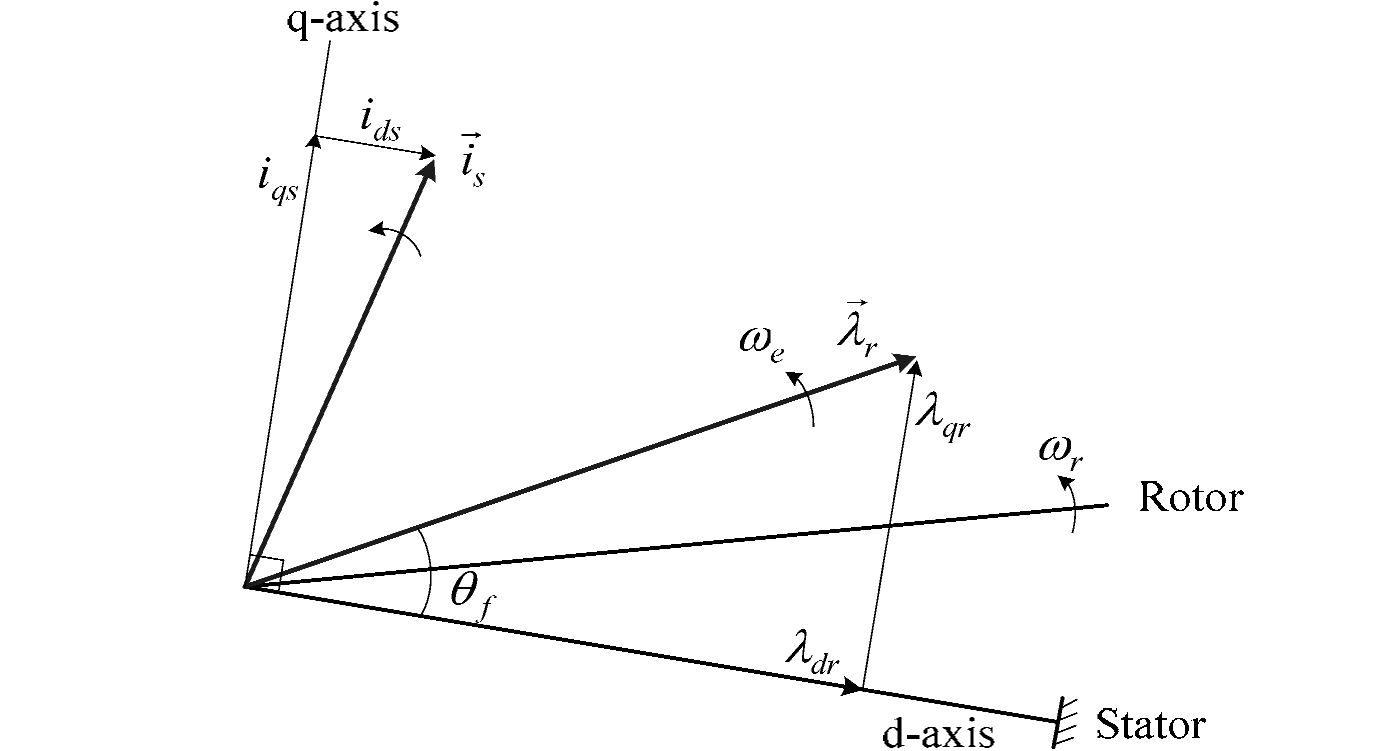
\includegraphics{graficos/img14.jpg} 
    \caption{Figura 14.5-2: Diagrama vectorial para \( \vec{\lambda_r} \) y \( \vec{i_s} \) utilizado en el calculador de flujo del rotor.}
    \label{fig:14.5-2}
\end{figure}
\FloatBarrier

La Figura 14.5-3 muestra el diagrama de bloques para la implementación digital del Calculador de Flujo del Rotor. De las tres tensiones del estator \( v_{as}, v_{bs} \) y \( v_{cs} \), solo se necesitan medir dos y la tercera se puede encontrar a partir de \( v_{as} + v_{bs} + v_{cs} = 0 \). Para reducir el número de sensores de tensión, las tensiones del estator también se pueden reconstruir utilizando la función de conmutación del inversor y la tensión de CC medida. Las tensiones y corrientes del estator se transforman luego en variables bifásicas a través de la transformación estacionaria 3/2. Los otros bloques se derivan de las ecuaciones (14.5-1) a (14.5-5). La salida del Calculador de Flujo del Rotor es el ángulo de flujo del rotor \( \theta_r \) y su amplitud \( \lambda_r \).

\begin{figure}[ht]
    \centering
    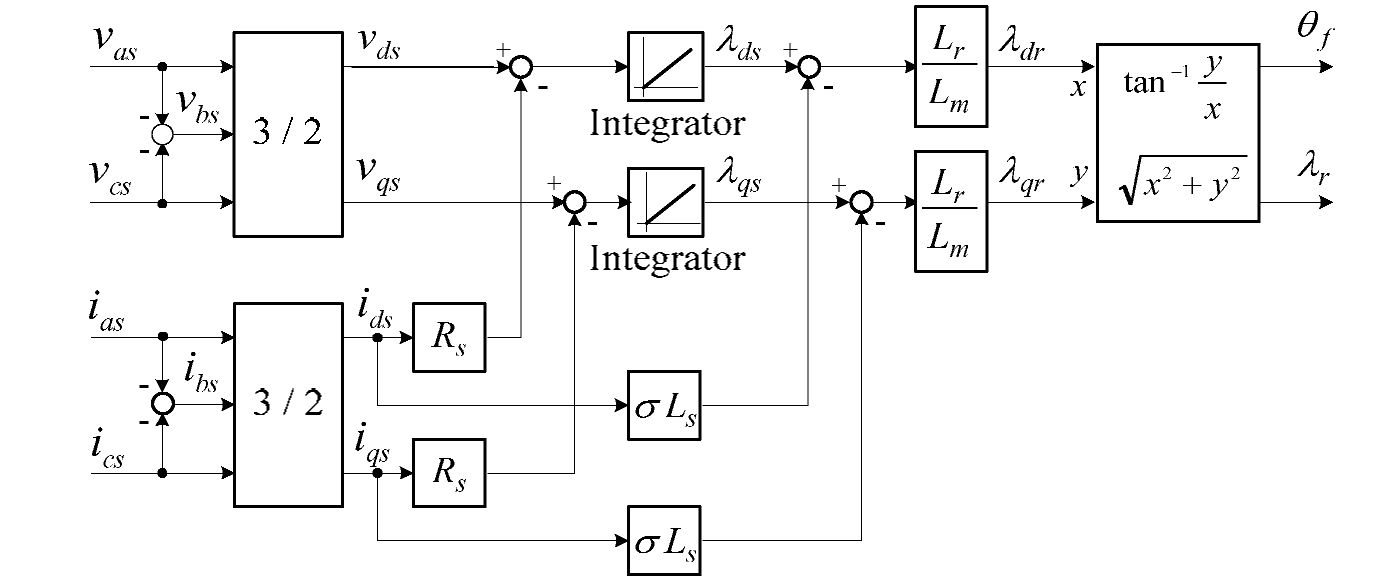
\includegraphics{graficos/img15.jpg} 
    \caption{Figura 14.5-3: Diagrama de bloques para el cálculo del flujo del rotor.}
    \label{fig:14.5-3}
\end{figure}
\FloatBarrier

\subsection{FOC Directo con VSI Controlado por Corriente}

El esquema FOC directo discutido en las secciones anteriores se puede simplificar si se utiliza un inversor de fuente de tensión controlado por corriente. La Figura 14.5-4 muestra el diagrama de bloques de dicho sistema. El VSI controlado por corriente puede hacer que las corrientes de salida del inversor \( i_{as}, i_{bs} \) e \( i_{cs} \) sigan sus referencias \( i_{as}^*, i_{bs}^* \) e \( i_{cs}^* \) de cerca. Por lo tanto, no es necesario usar los controladores de corriente en la Fig. 14.5-1. Además, el esquema PWM para el VSI regulado por corriente es más simple que otras técnicas de modulación.


\begin{figure}[ht]
    \centering
    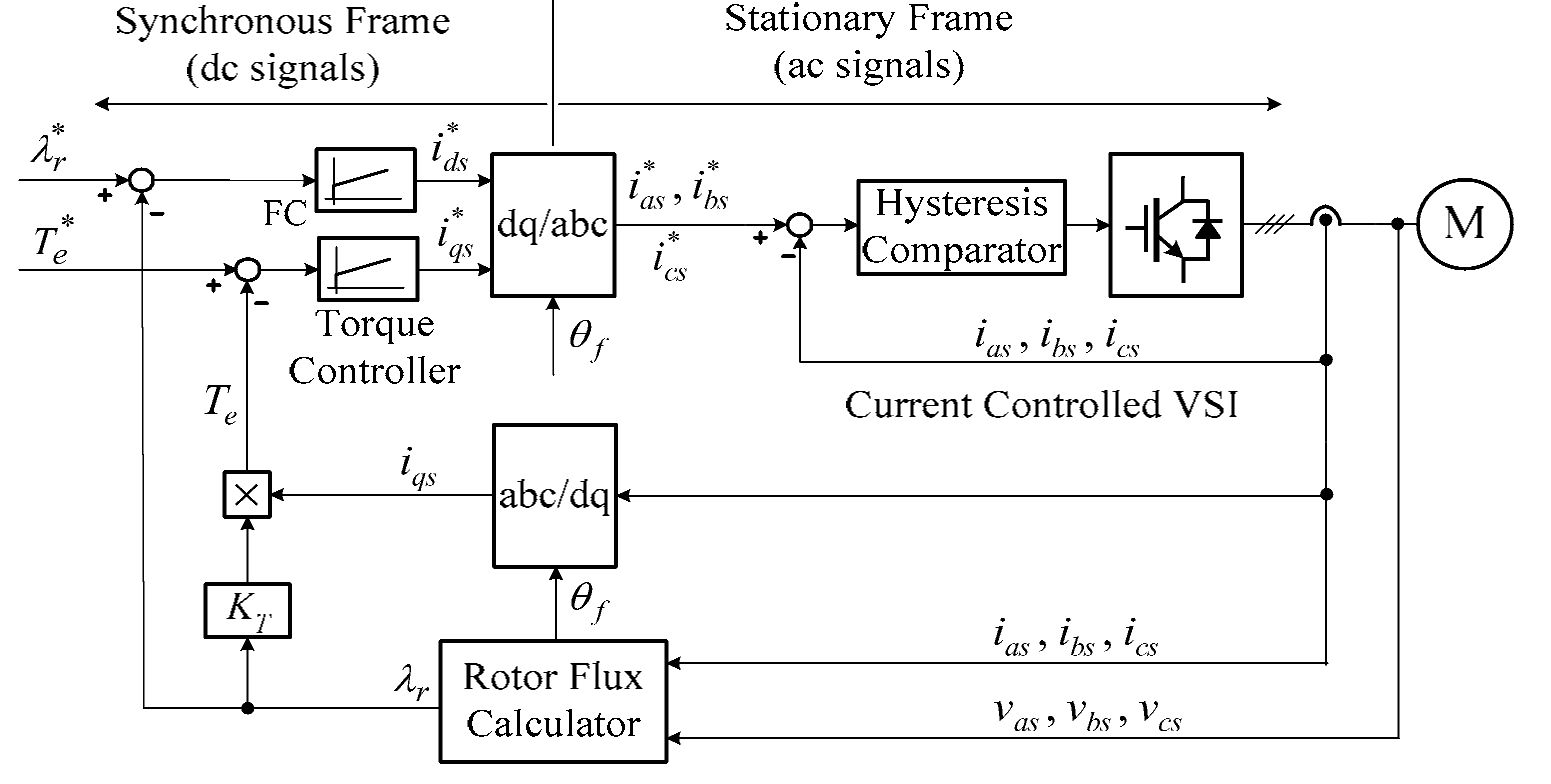
\includegraphics{graficos/img16.jpg} 
    \caption{Figura 14.5-4: FOC directo con un VSI controlado por corriente.}
    \label{fig:14.5-4}
\end{figure}
\FloatBarrier


El principio de funcionamiento del VSI regulado por corriente se ilustra en la Fig. 14.5-5, donde se muestra el control de solo una de las tres corrientes de fase. La corriente de salida del inversor \( i_{as} \) se mide y se compara con su referencia \( i_{as}^* \). Su diferencia \( \Delta i \) se envía a un comparador de histéresis. La salida del comparador \( x_H \) es lógica '1' o '0', en función de la cual se generan las señales de compuerta para los interruptores \( S_1 \) y \( S_4 \). El comparador de histéresis tiene una banda de tolerancia de \( \delta \).

Supongamos que la corriente de referencia \( i_{as}^* \) es sinusoidal, como se ilustra en la Fig. 14.5-5b. La corriente de salida del inversor \( i_{as} \) se mantiene dentro de los límites superior e inferior establecidos por \( \delta \). Suponiendo que \( x_H \) se vuelve lógica '1' en el instante \( t_1 \), \( S_1 \) se enciende y \( S_4 \) se apaga. La tensión terminal del inversor \( v_{AN} \) es igual a la tensión de CC \( V_d \), lo que hace que \( i_{as} \) aumente. La tasa de aumento de corriente está determinada principalmente por \( V_d \), los parámetros del motor y su fuerza contraelectromotriz. Cuando \( i_{as} \) alcanza su límite superior en \( t_2 \), \( x_H \) se vuelve lógica '0', lo que lleva al apagado de \( S_1 \) y encendido de \( S_4 \). La \( v_{AN} \) resultante es cero, lo que hace que \( i_{as} \) disminuya. Cuando \( i_{as} \) alcanza el límite inferior en \( t_3 \), \( x_H \) se vuelve '0', \( v_{AN} = V_d \) y \( i_{as} \) comienza a aumentar nuevamente. Como resultado, \( i_{as} \) se mantiene dentro de los límites superior e inferior. Para hacer que \( i_{as} \) siga más de cerca su referencia \( i_{as}^* \) con menos armónicas de conmutación, se puede reducir la banda \( \delta \). Sin embargo, esto se logra a expensas de un aumento en la frecuencia de conmutación.

Para un \( \delta \) y \( V_d \) dados, la frecuencia de conmutación del inversor puede variar con los parámetros del motor. Esto se considera como una desventaja mayor del inversor regulado por corriente con el control de banda de tolerancia. Cuando el inversor utiliza otras técnicas de modulación como SPWM y SVM, su frecuencia de conmutación está determinada por el esquema de modulación, independientemente de los parámetros del motor.

\begin{figure}[ht]
    \centering
    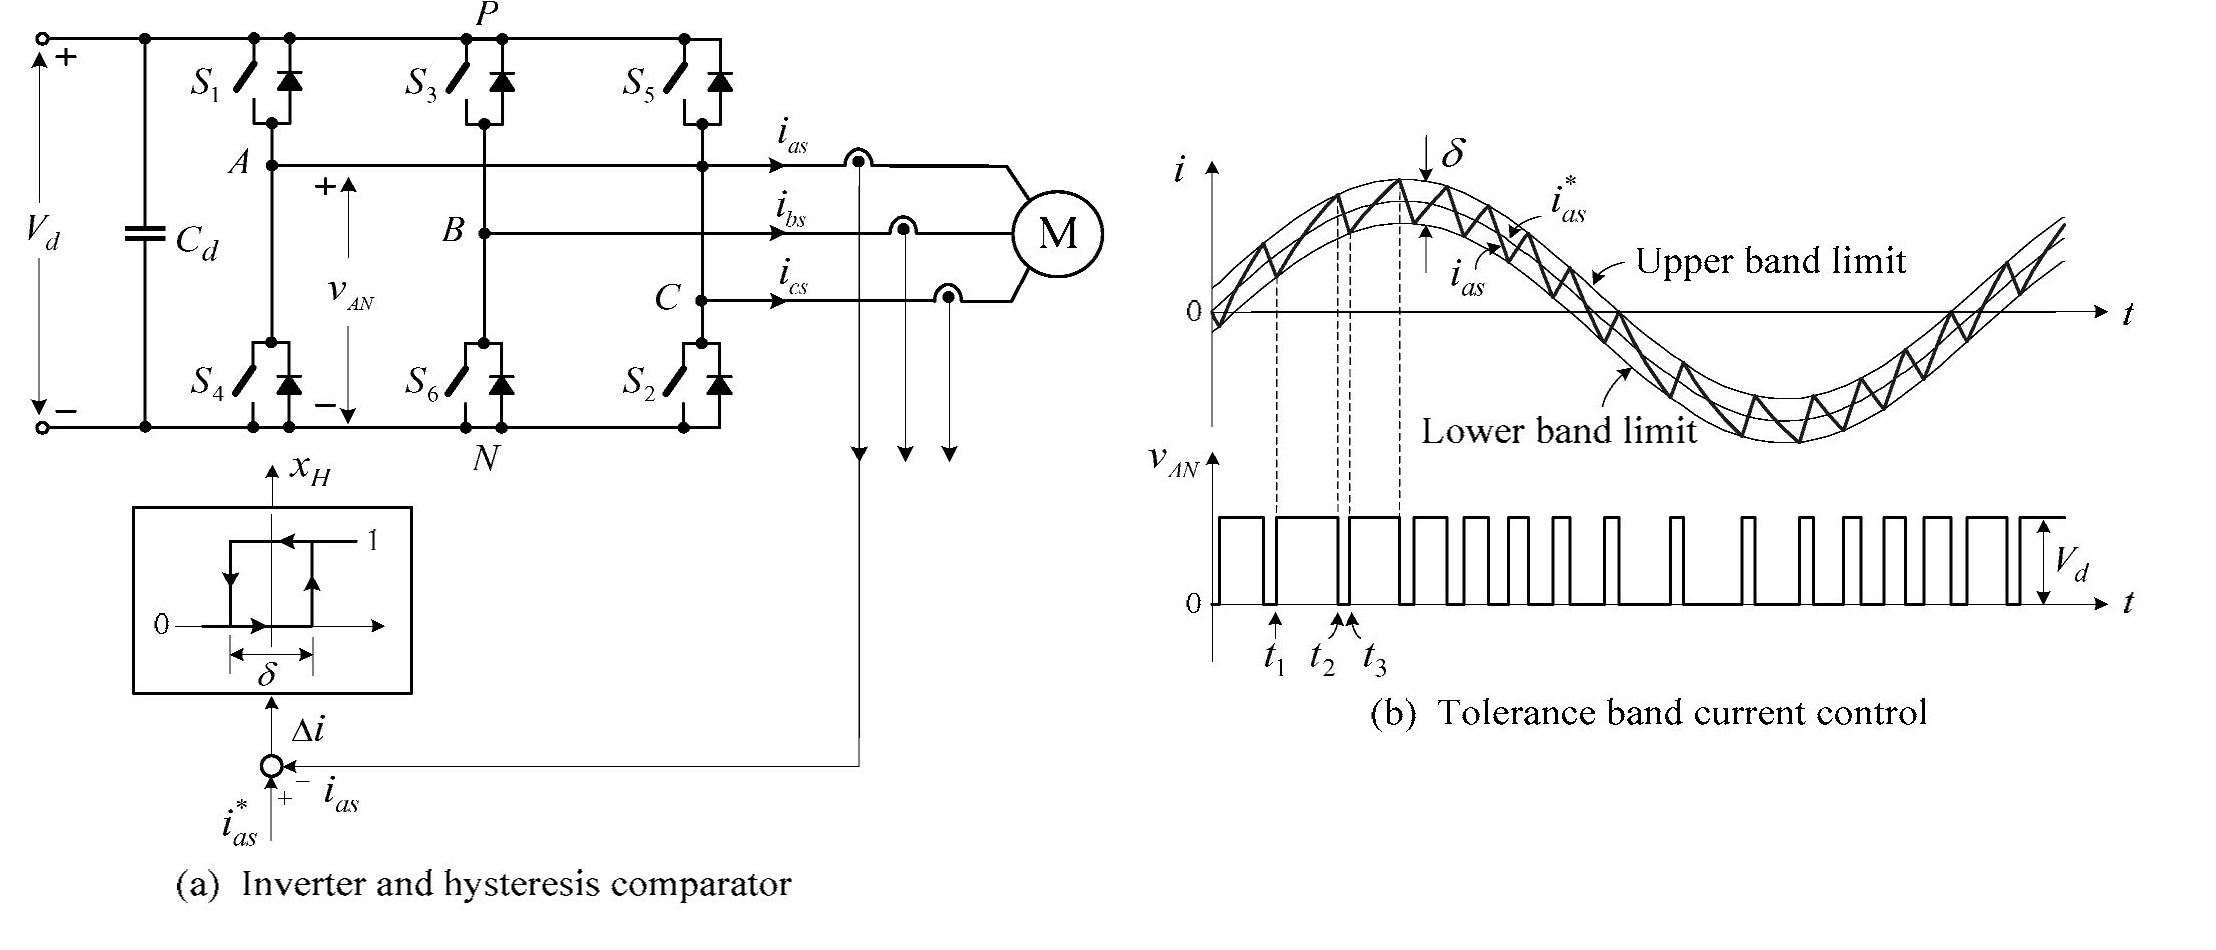
\includegraphics{graficos/img17.jpg} 
    \caption{Figura 14.5-5: Inversor y comparador de histéresis.}
    \label{fig:14.5-5}
\end{figure}
\FloatBarrier

La Figura 14.5-6 muestra las formas de onda simuladas para un accionamiento de motor de inducción utilizando el esquema FOC directo. El diagrama de bloques del sistema de accionamiento se muestra en la Fig. 14.5-4, donde no se muestra el bucle de control de velocidad. Los datos y parámetros de la placa de identificación del motor se enumeran en la Tabla 14.5-1.

La banda de tolerancia \( \delta \) del comparador de histéresis se ajusta de tal manera que la frecuencia de conmutación del inversor es de alrededor de 600 Hz. La referencia de flujo del rotor \( \lambda_r^* \) se establece en su valor nominal de 8.35 Wb. El par máximo se limita a su valor nominal de 7490 N·m durante los transitorios del motor.

El motor opera inicialmente a una velocidad de rotor de \( n_r = 200 \) rpm. La referencia de velocidad \( n_r^* \) tiene un aumento escalonado de 200 rpm a la velocidad nominal del rotor de 1189 rpm en el instante de tiempo \( t = 0.1 \) s. El motor acelera sin carga mientras su par se limita al valor nominal. El par contiene altas ondulaciones debido a la baja frecuencia de conmutación. La corriente del estator \( i_{as} \) aumenta a su valor nominal durante el transitorio. Cuando \( n_r \) alcanza su referencia de 1189 rpm alrededor de \( t = 0.4 \) s, el \( T_e \) promedio cae a cero, y \( i_{as} \) se reduce a un valor que corresponde a la corriente de magnetización del motor. Debido al control desacoplado de flujo y par por el esquema FOC, el

\begin{figure}[ht]
    \centering
    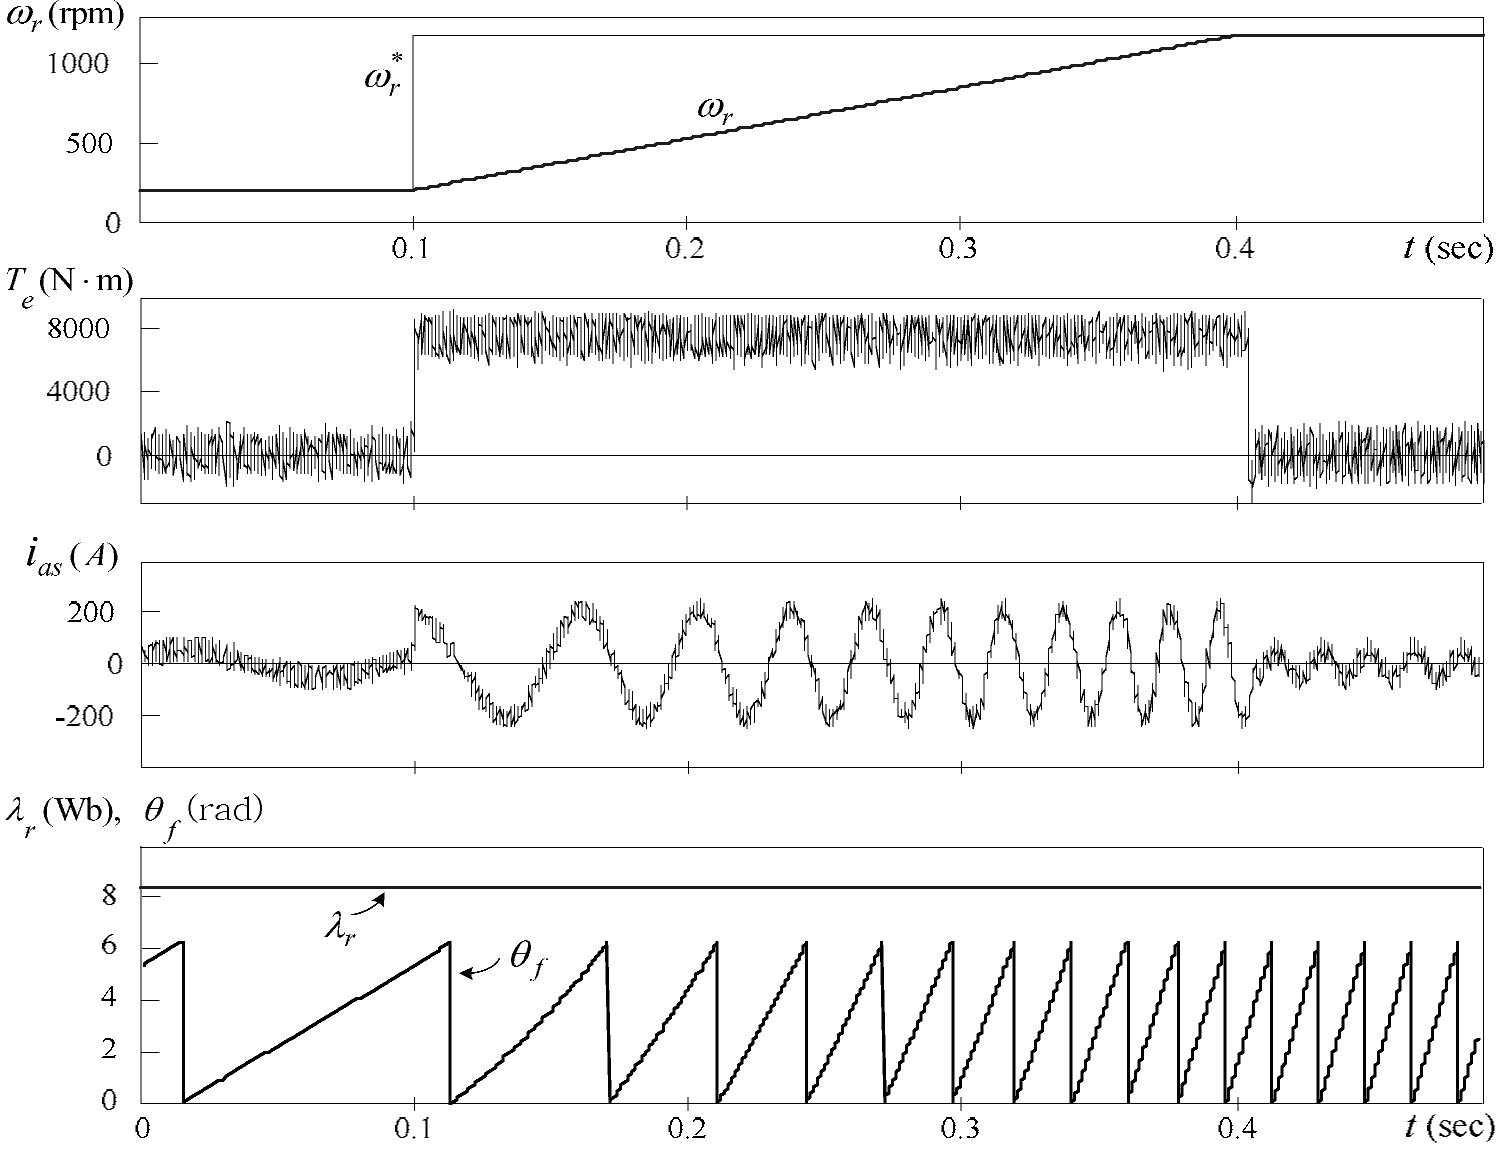
\includegraphics{graficos/img18.jpg} 
    \caption{Figura 14.5-6: Formas de onda simuladas para un accionamiento de motor de inducción con el esquema FOC directo.}
    \label{fig:14.5-6}
\end{figure}
\FloatBarrier

\begin{table}[ht]
    \centering
    \caption{Tabla 14.5-1: Datos y parámetros de la placa de identificación del motor}
    \begin{tabular}{|l|c|}
        \hline
        \textbf{Calificaciones del Motor} & \textbf{Parámetros del Motor} \\
        \hline
        Potencia nominal de salida & 1250 hp \\
        Tensión nominal entre líneas & 4160 V \\
        Corriente nominal del estator & 150 A \\
        Velocidad nominal & 1189 rpm \\
        Par nominal & 7490 N·m \\
        Enlace de flujo nominal del estator & 9.0 Wb \\
        Enlace de flujo nominal del rotor & 8.35 Wb \\
        \hline
        Resistencia del estator, \( R_s \) & 0.21 \(\Omega\) \\
        Resistencia del rotor, \( R_r \) & 0.146 \(\Omega\) \\
        Inductancia de fuga del estator, \( L_{ls} \) & 5.2 mH \\
        Inductancia de fuga del rotor, \( L_{lr} \) & 5.2 mH \\
        Inductancia de magnetización, \( L_m \) & 155 mH \\
        Momento de inercia, \( J \) & 22 kg·m² \\
        \hline
    \end{tabular}
    \label{tab:14.5-1}
\end{table}
\FloatBarrier


\end{document}